\subsection{Kinematic Distributions}
\label{sec:kinematic_distributions}

The distributions below use the nominal $e'p\pi^-$ sample after the particle identification, fiducial and exclusivity selections described above. The underlying DIS requirements are
\begin{align}
 Q^2 &\geq 1~\mathrm{GeV}^2, \\
 W &\geq 2~\mathrm{GeV}, \\
 y &\leq 0.80.
 \label{eq:eppi_kinematic_requirements}
\end{align}
The outbending RGB fall-2019 sample additionally requires $Q^2>1.5$~GeV$^2$ to better match the low-$Q^2$ coverage of the inbending samples. These requirements are imposed before the exclusivity calibration and remain part of the nominal selection. The displayed sample lies within $0.10\leq x_B<0.60$ and $0.05\leq-t'<1.25$~GeV$^2$.


Figure~\ref{fig:eppi_kin_comparison} compares the principal RGB and RGC shapes directly. Both samples cover broad, overlapping regions of $x_B$, $Q^2$, $W$, $-t'$ and $y$, with visible differences in their populations and azimuthal coverage. Their correlations are shown in Figs.~\ref{fig:eppi_kin_rgb_core} and~\ref{fig:eppi_kin_rgc_core}.

The correlations of $Q^2$, $x_B$ and $-t'$ with the pion production azimuth $\phi$ are shown in Figs.~\ref{fig:eppi_kin_rgb_phi_correlations} and~\ref{fig:eppi_kin_rgc_phi_correlations}. Figures~\ref{fig:eppi_kin_rgb_phi_projections} and~\ref{fig:eppi_kin_rgc_phi_projections} show the corresponding projections in the four $x_B$ intervals. The azimuthal population is nonuniform and depends on the sampled kinematics. 

The $Q^2$ distributions in the 24 $(x_B,-t')$ bins are shown in Figs.~\ref{fig:eppi_kin_rgb_Q2} and~\ref{fig:eppi_kin_rgc_Q2}. Each panel fixes one $-t'$ interval and overlays the four $x_B$ intervals. These distributions characterize the finite kinematic extent of each bin and the different weights with which RGB and RGC sample that region.

Figures~\ref{fig:eppi_kin_rgb_pion} and~\ref{fig:eppi_kin_rgc_pion} show the detected $\pi^-$ momentum distributions. Here each panel fixes an $x_B$ interval and the six colored curves represent the $-t'$ intervals. The momentum range and distribution shape change across the analysis bins.

The detected-proton momentum and angular distributions are shown separately for FD and CD reconstruction. These are selected candidate populations rather than detector efficiencies. The current selected sample counts are given in Table~\ref{tab:release_counts}. The displayed distributions retain the fine selection bins, including for the merged target-spin analysis.
\FloatBarrier

\begin{figure}[p]
\centering
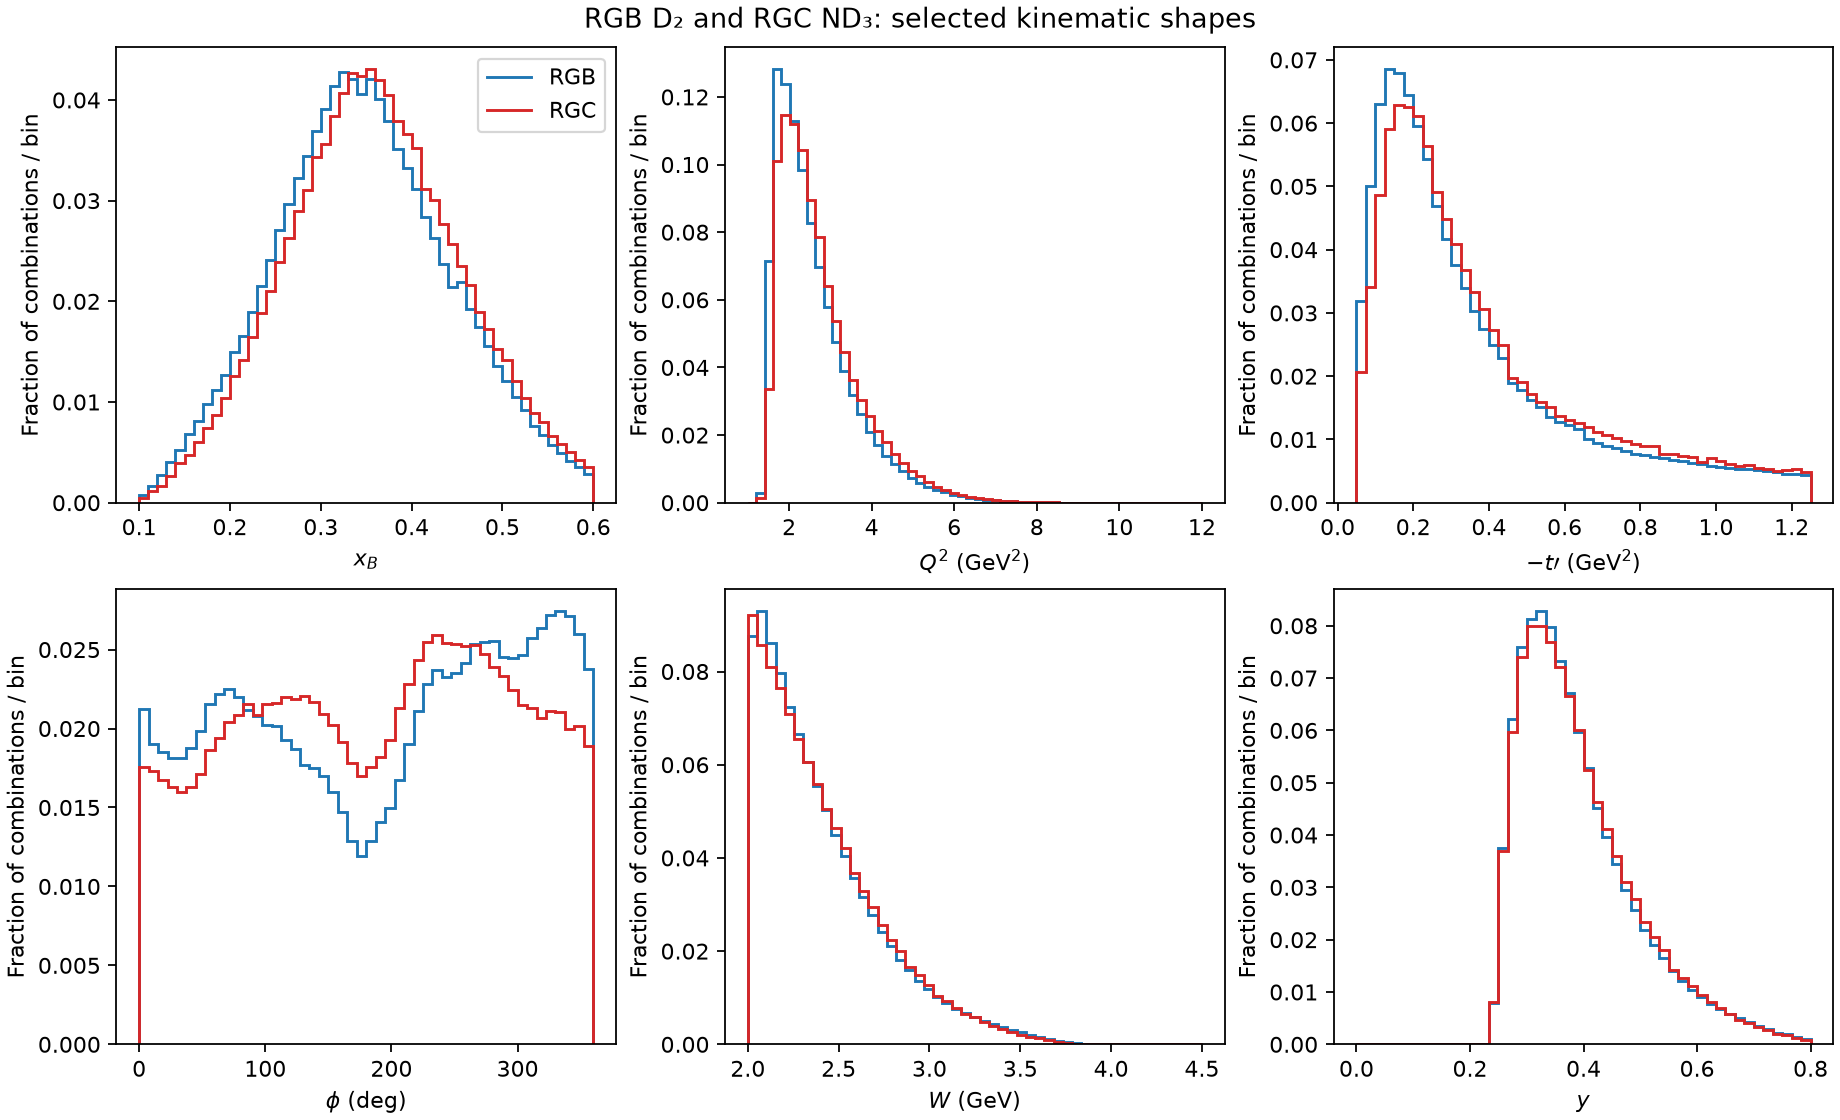
\includegraphics[width=0.98\linewidth]{figures/channel_selection/kinematic_distributions/RGB_RGC_shape_comparison.png}
\caption{Comparison of the nominal RGB D$_2$ (blue) and RGC ND$_3$ (red) kinematic shapes. Each distribution is independently normalized to unit population in its displayed range.}
\label{fig:eppi_kin_comparison}
\end{figure}
\clearpage

% \begin{figure}[p]
% \centering
% 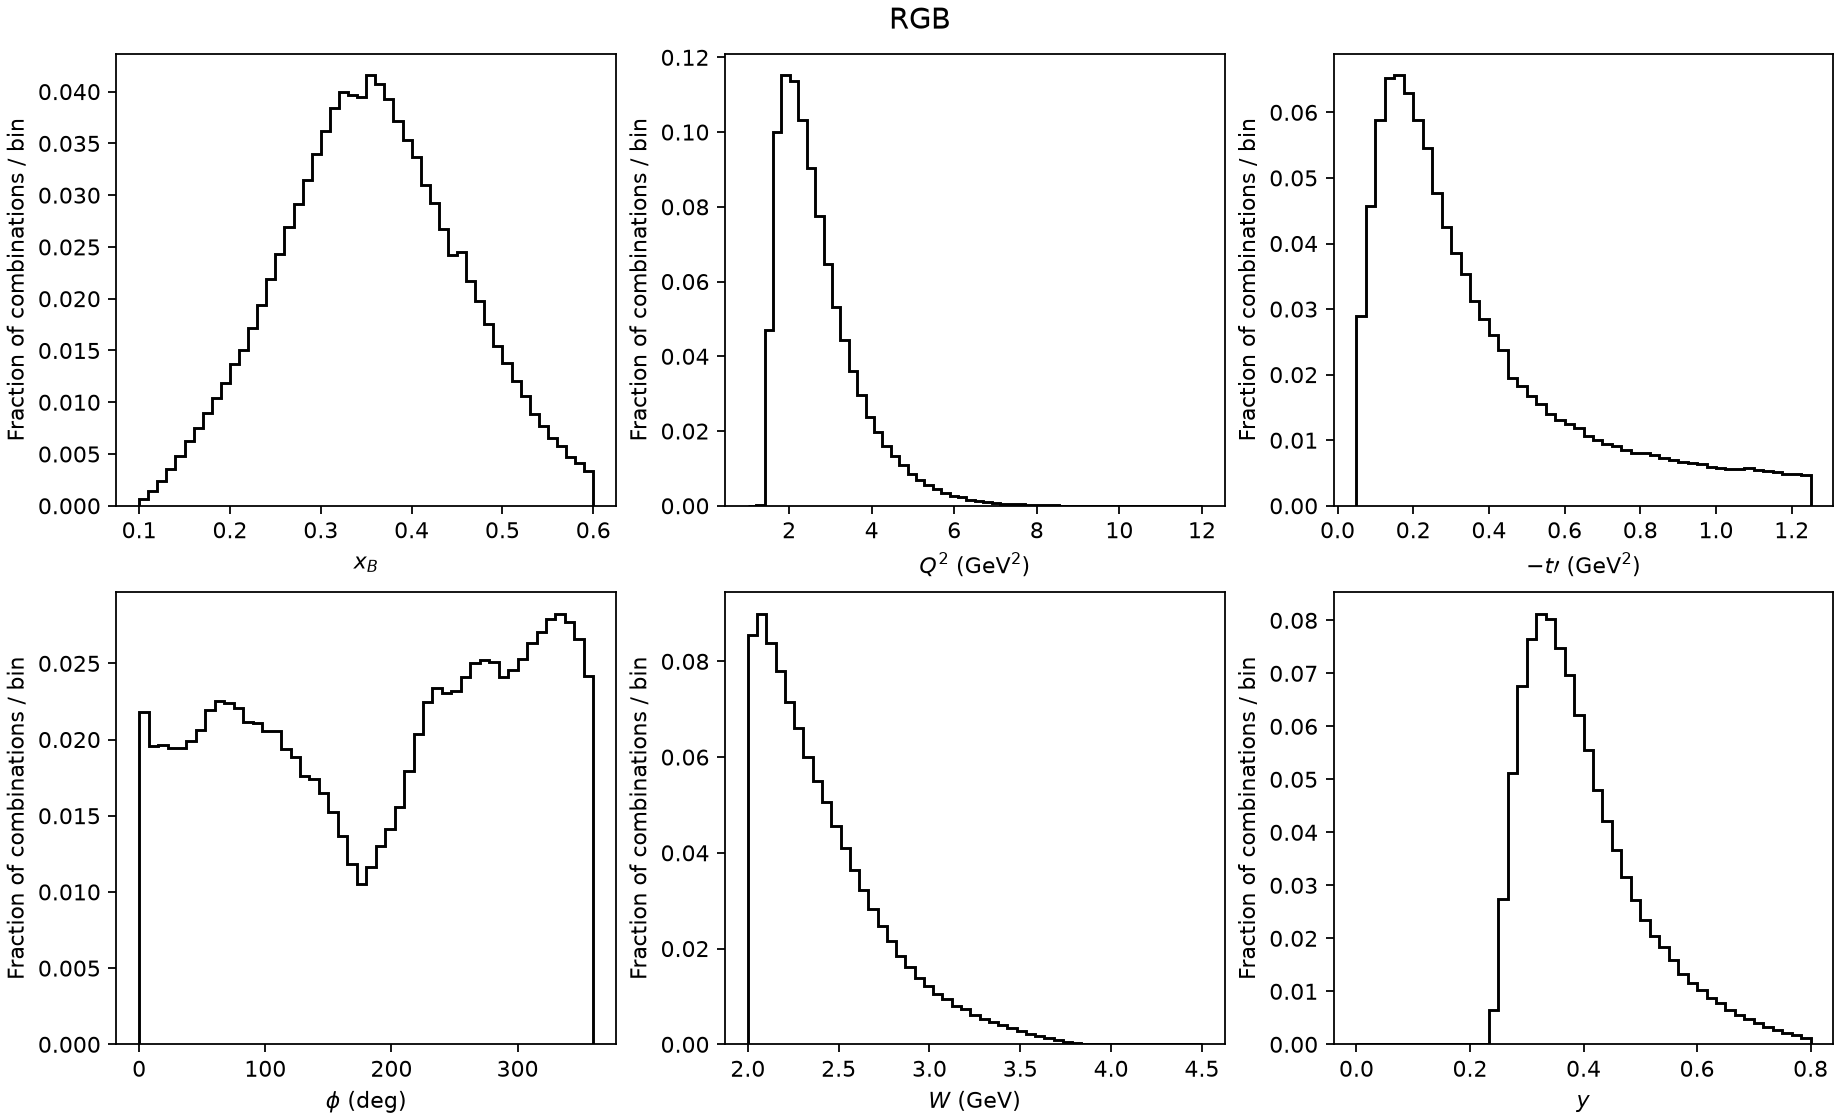
\includegraphics[width=0.98\linewidth]{figures/channel_selection/kinematic_distributions/RGB/01_kinematic_1d.png}
% \caption{RGB D$_2$: One-dimensional distributions of $x_B$, $Q^2$, $-t^\prime$, pion production azimuth $\phi$, $W$ and $y$ for the nominally selected sample. Each distribution is normalized to unit population in its displayed range.}
% \label{fig:eppi_kin_rgb_1d}
% \end{figure}

% \begin{figure}[p]
% \centering
% 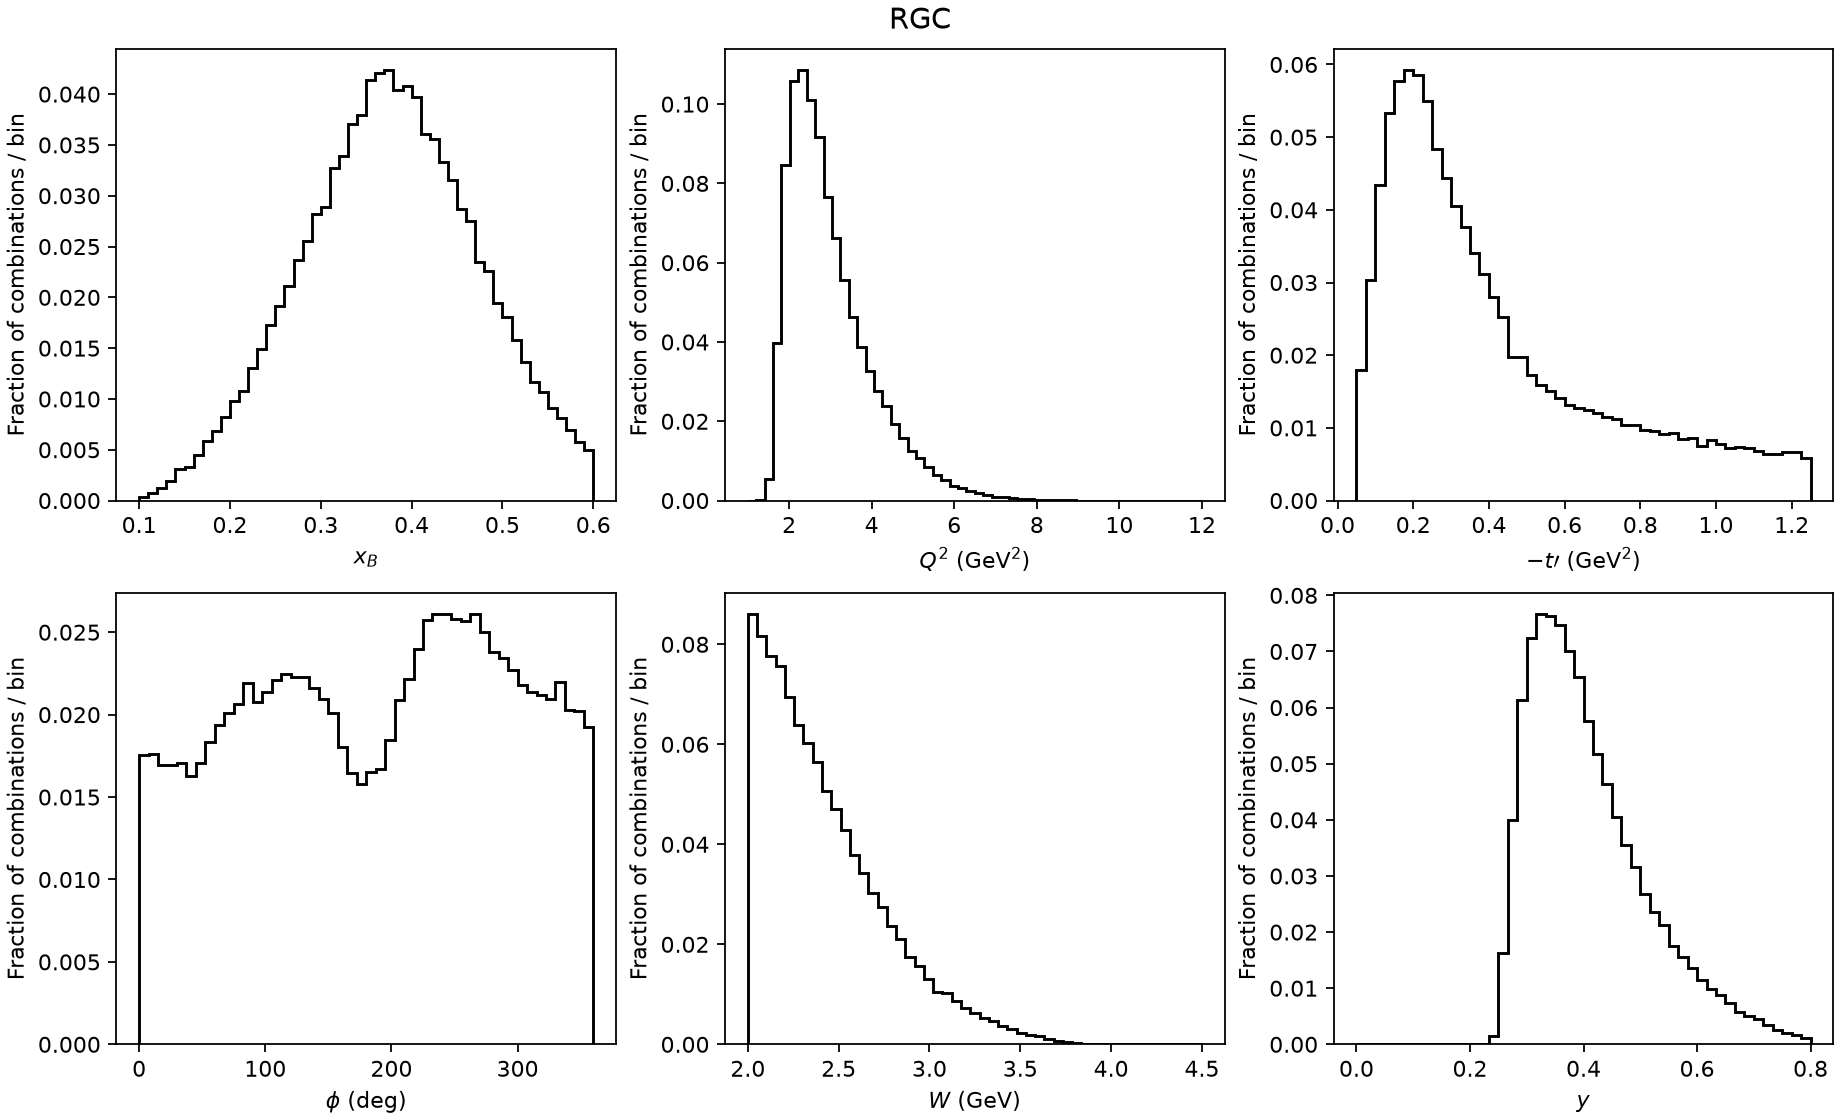
\includegraphics[width=0.98\linewidth]{figures/channel_selection/kinematic_distributions/RGC/01_kinematic_1d.png}
% \caption{RGC ND$_3$: One-dimensional distributions of $x_B$, $Q^2$, $-t^\prime$, pion production azimuth $\phi$, $W$ and $y$ for the nominally selected sample. Each distribution is normalized to unit population in its displayed range.}
% \label{fig:eppi_kin_rgc_1d}
% \end{figure}
% \clearpage

\begin{figure}[p]
\centering
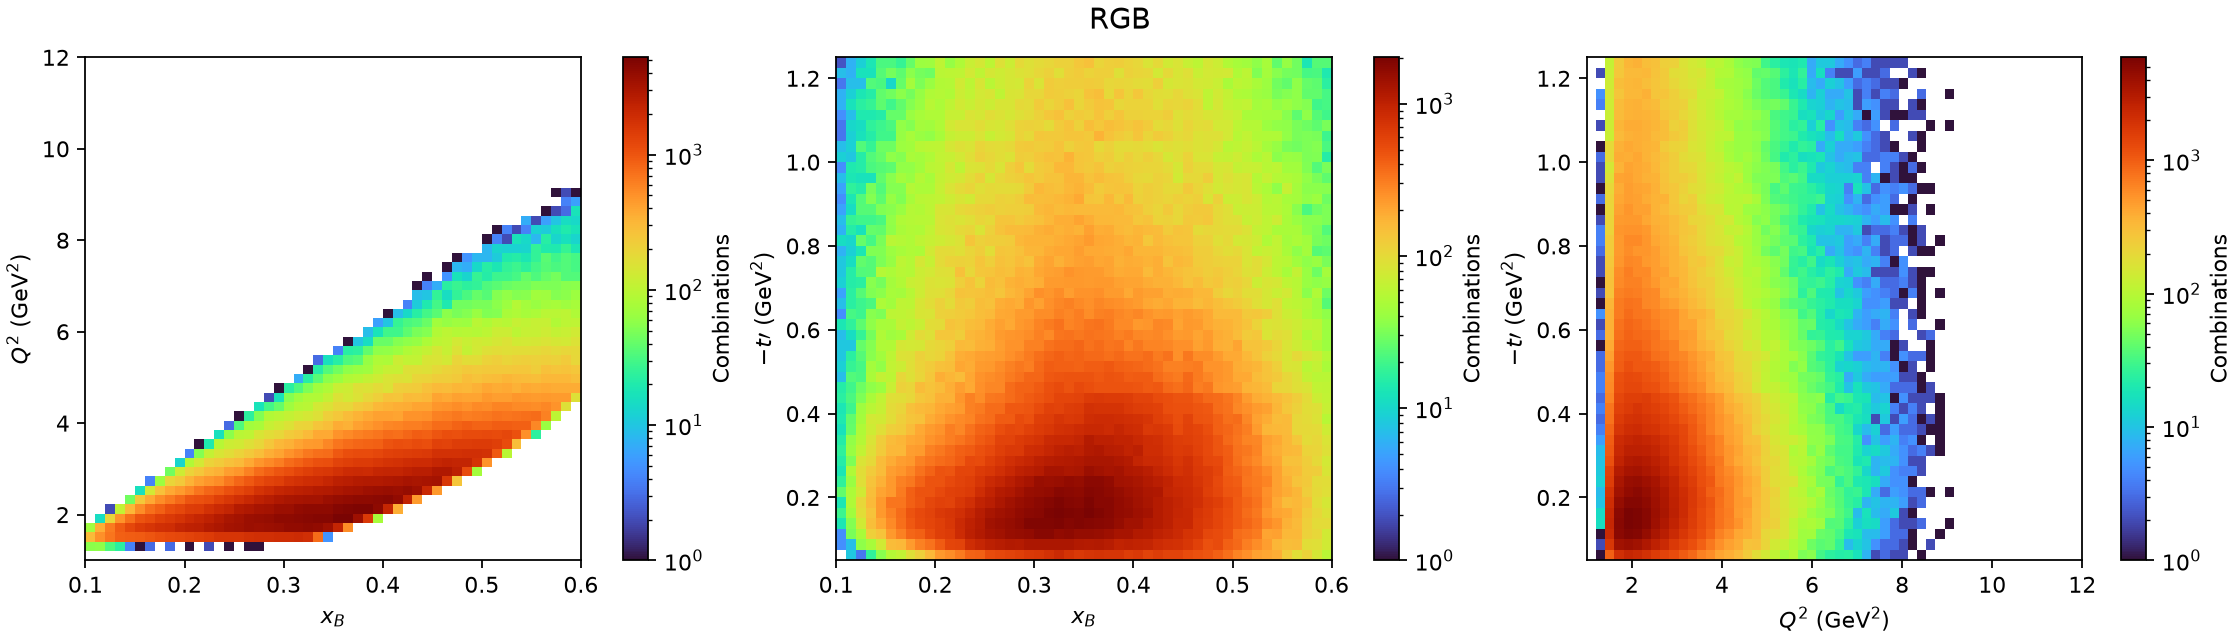
\includegraphics[width=0.98\linewidth]{figures/channel_selection/kinematic_distributions/RGB/02_core_correlations.png}
\caption{RGB D$_2$: Correlations among $x_B$, $Q^2$ and $-t^\prime$ for the nominally selected sample.}
\label{fig:eppi_kin_rgb_core}
\end{figure}

\begin{figure}[p]
\centering
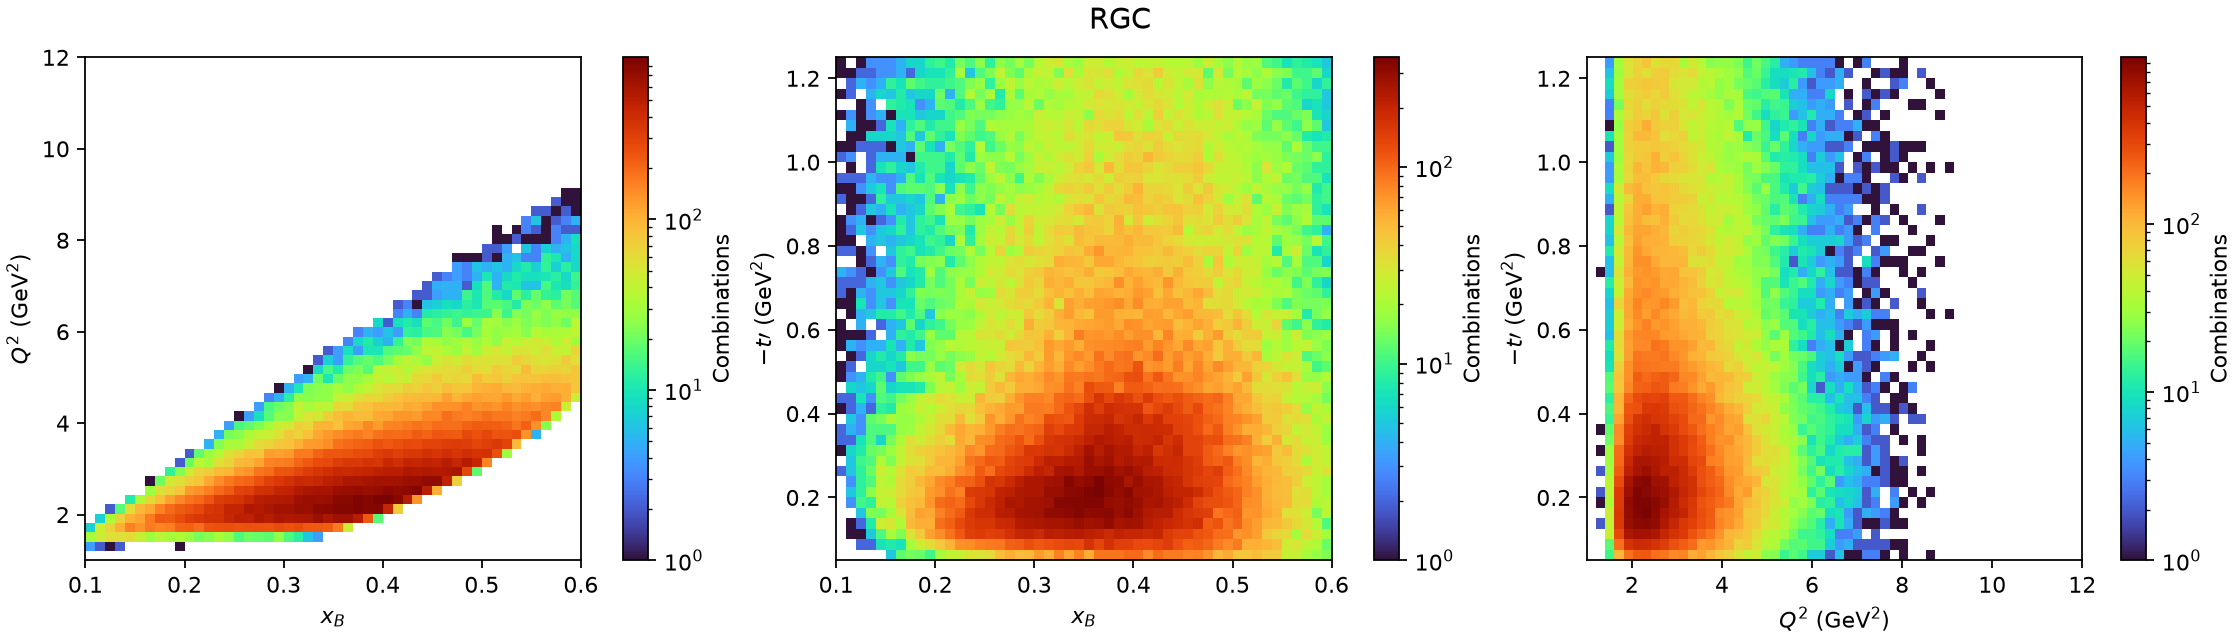
\includegraphics[width=0.98\linewidth]{figures/channel_selection/kinematic_distributions/RGC/02_core_correlations.png}
\caption{RGC ND$_3$: Correlations among $x_B$, $Q^2$ and $-t^\prime$ for the nominally selected sample.}
\label{fig:eppi_kin_rgc_core}
\end{figure}
\clearpage

\begin{figure}[p]
\centering
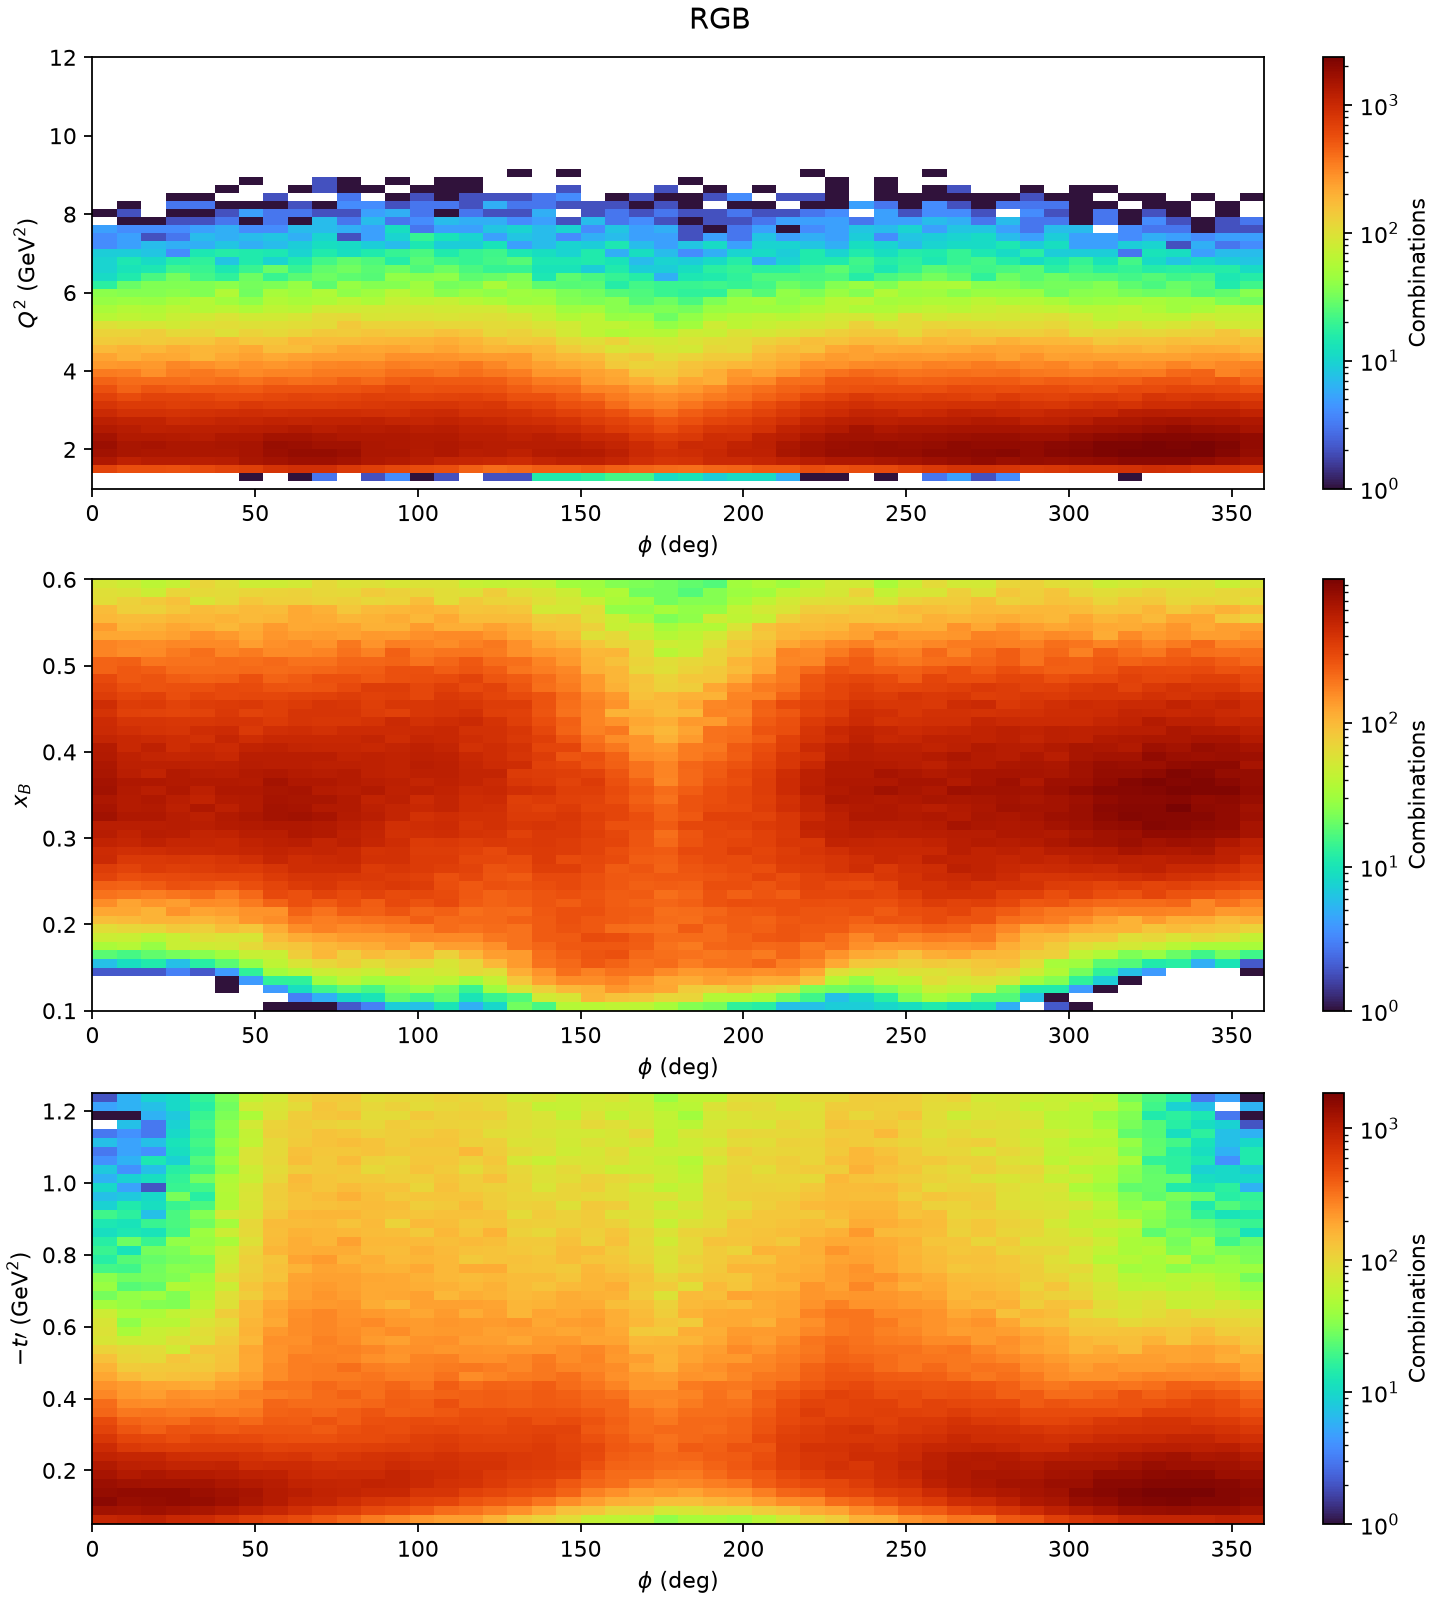
\includegraphics[width=0.85\linewidth]{figures/channel_selection/kinematic_distributions/RGB/03_phi_correlations.png}
\caption{RGB D$_2$: Correlations of $Q^2$, $x_B$ and $-t^\prime$ with the pion production azimuth $\phi$, displayed in degrees.}
\label{fig:eppi_kin_rgb_phi_correlations}
\end{figure}

\begin{figure}[p]
\centering
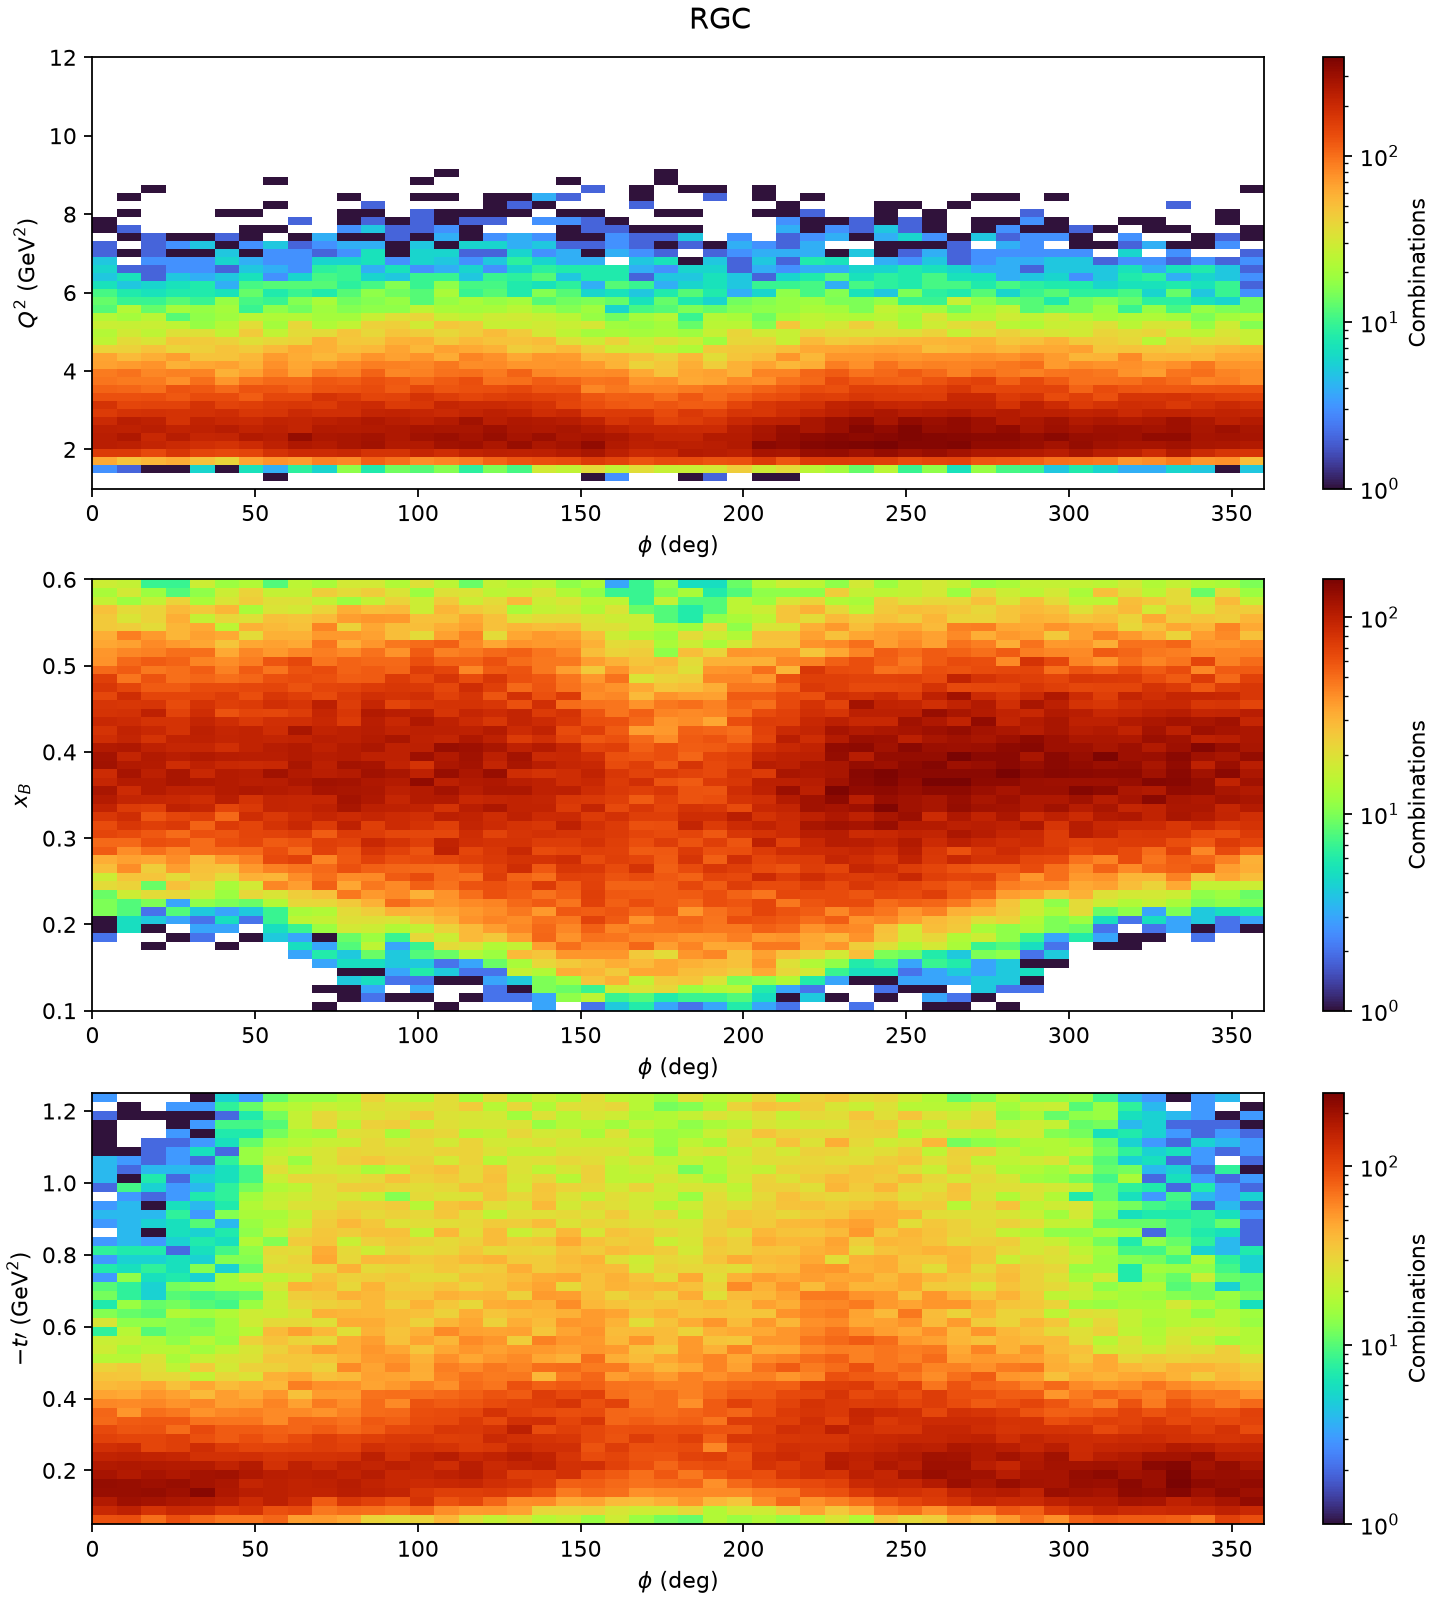
\includegraphics[width=0.85\linewidth]{figures/channel_selection/kinematic_distributions/RGC/03_phi_correlations.png}
\caption{RGC ND$_3$: Correlations of $Q^2$, $x_B$ and $-t^\prime$ with the pion production azimuth $\phi$, displayed in degrees.}
\label{fig:eppi_kin_rgc_phi_correlations}
\end{figure}
\clearpage

\begin{figure}[p]
\centering
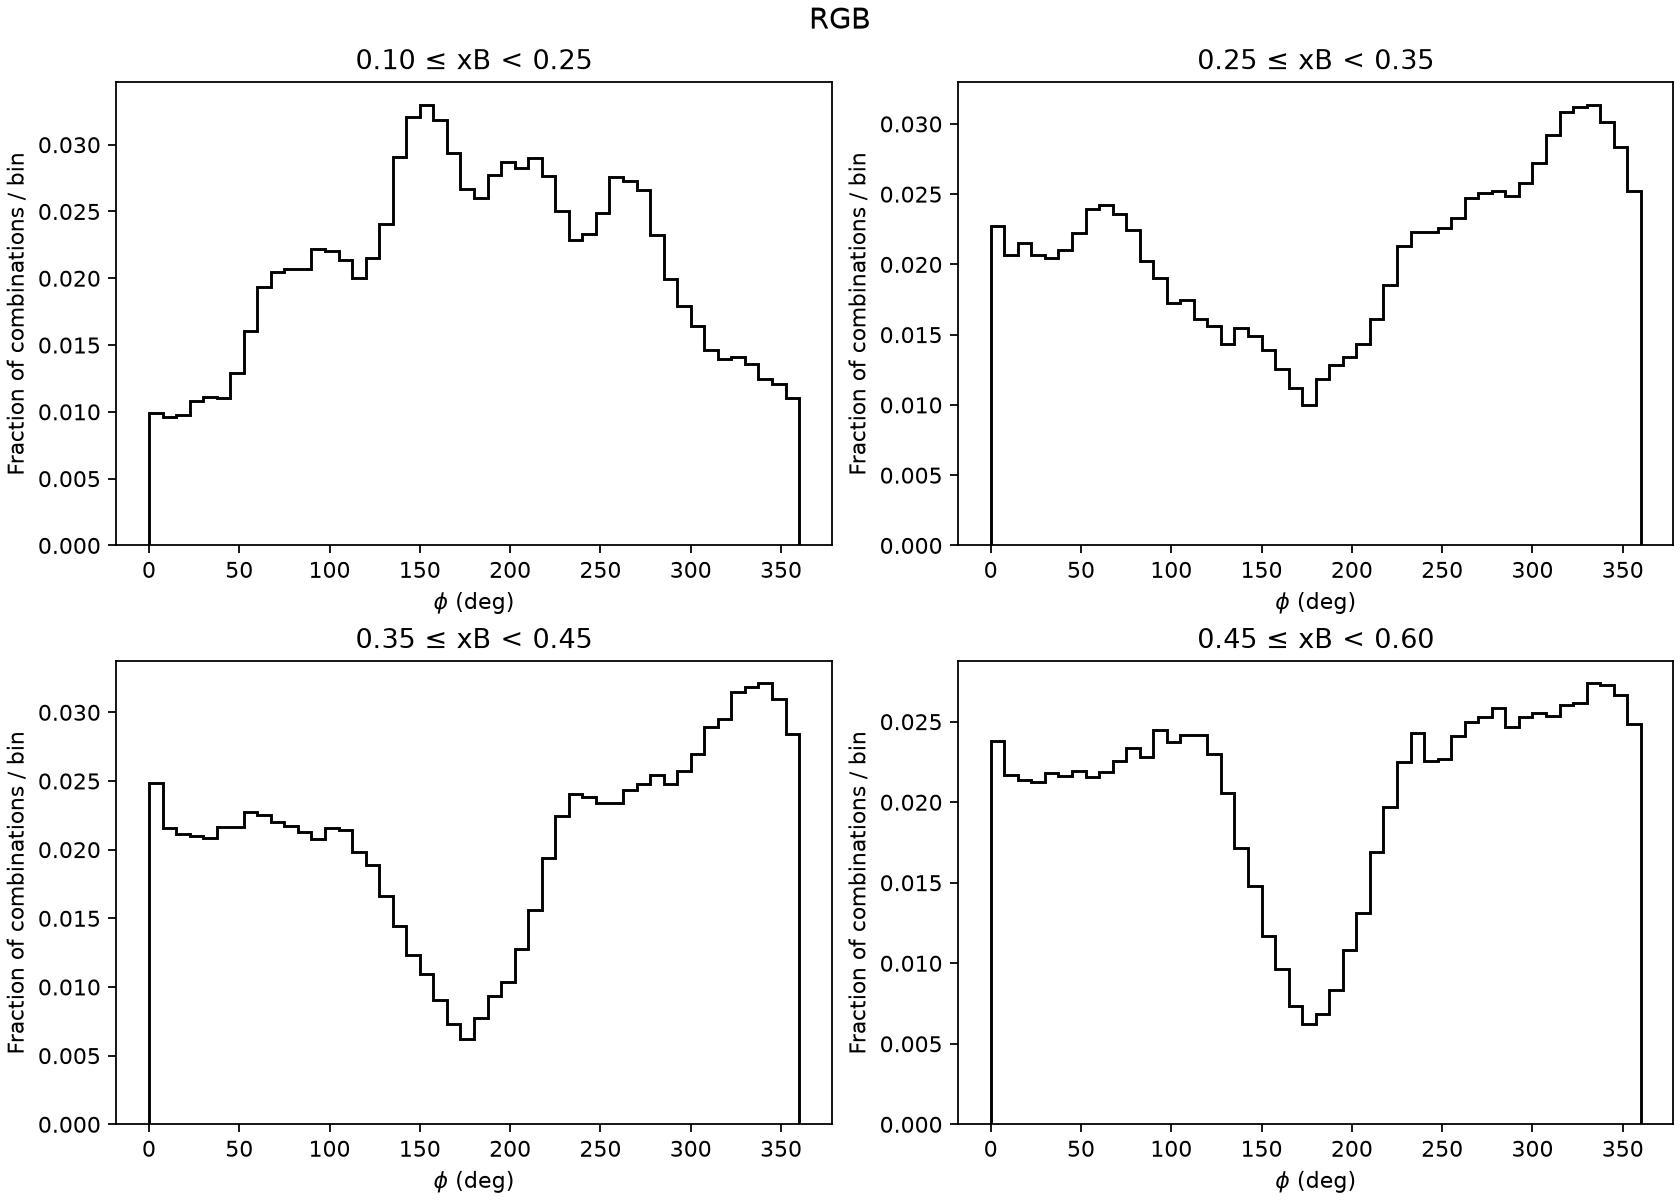
\includegraphics[width=0.98\linewidth]{figures/channel_selection/kinematic_distributions/RGB/04_phi_projections.png}
\caption{RGB D$_2$: Normalized one-dimensional $\phi$ projections in the four analysis $x_B$ intervals. These distributions show the nonuniform azimuthal population of the accepted sample.}
\label{fig:eppi_kin_rgb_phi_projections}
\end{figure}

\begin{figure}[p]
\centering
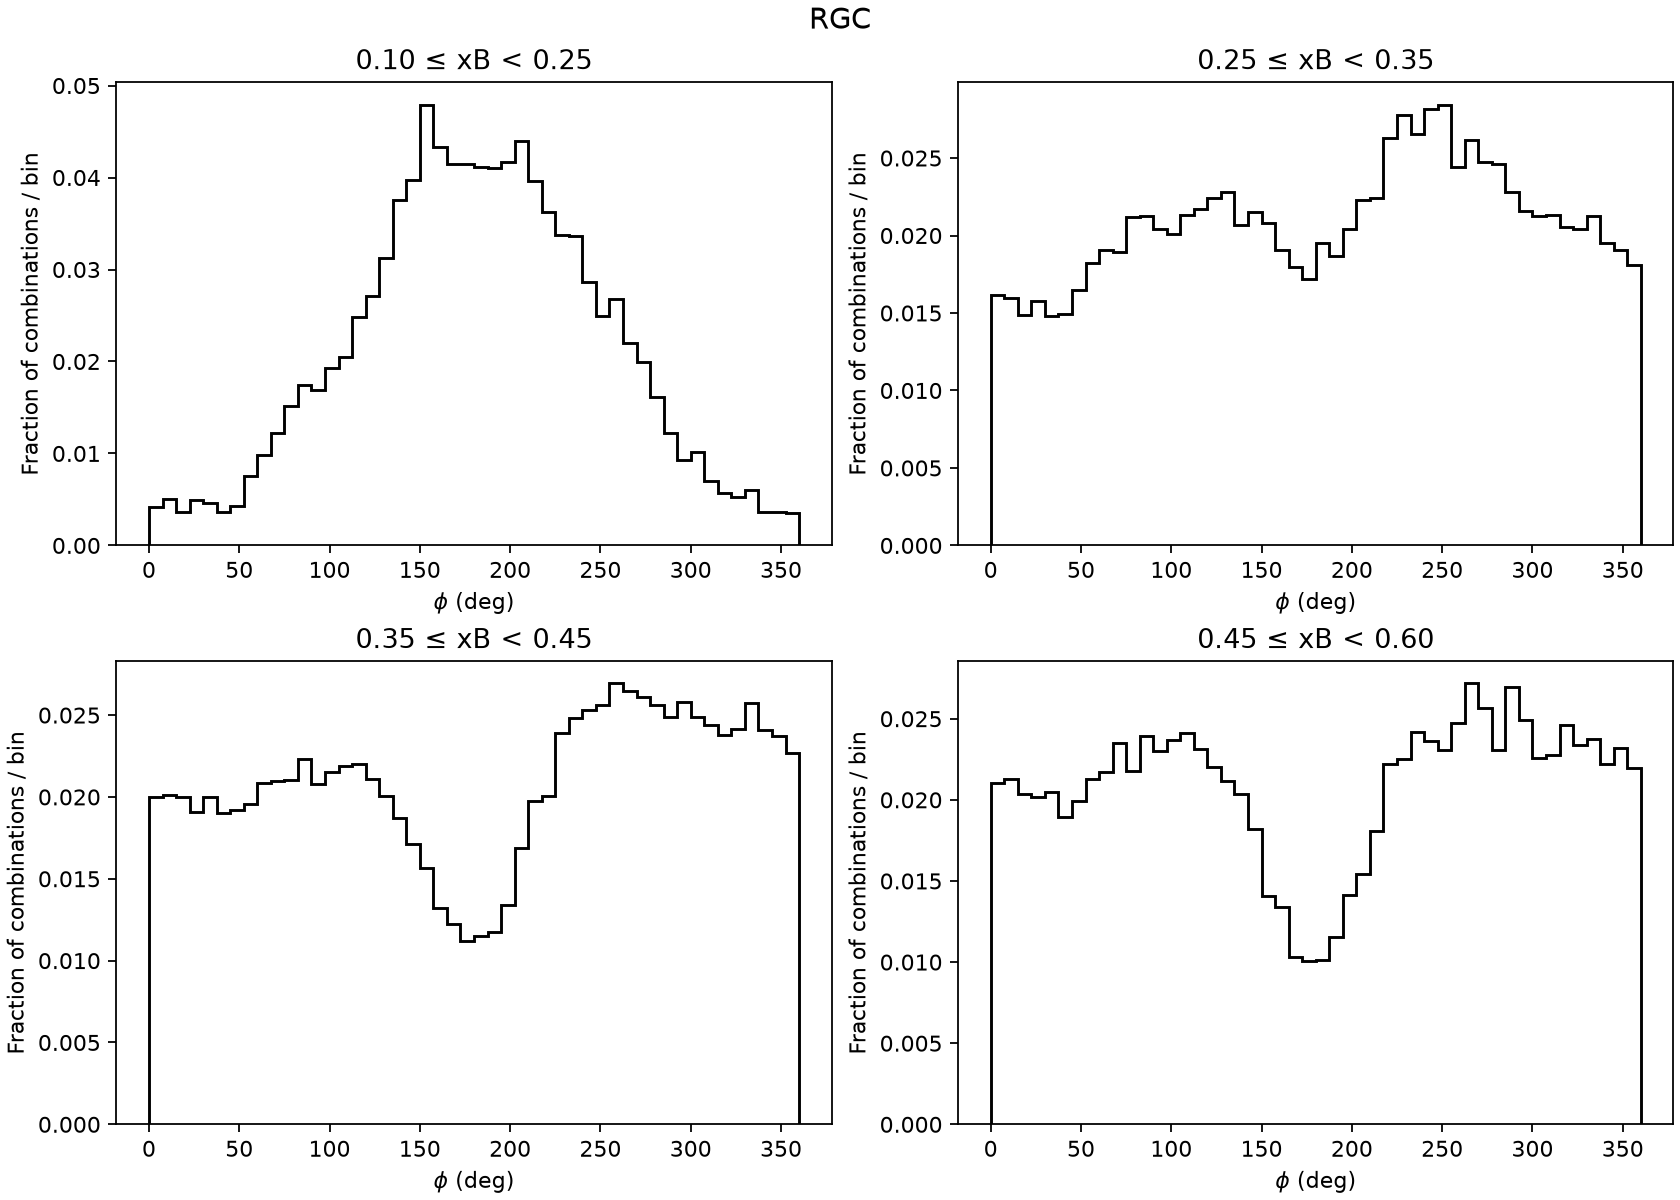
\includegraphics[width=0.98\linewidth]{figures/channel_selection/kinematic_distributions/RGC/04_phi_projections.png}
\caption{RGC ND$_3$: Normalized one-dimensional $\phi$ projections in the four analysis $x_B$ intervals. These distributions show the nonuniform azimuthal population of the accepted sample.}
\label{fig:eppi_kin_rgc_phi_projections}
\end{figure}
\clearpage

\begin{figure}[p]
\centering
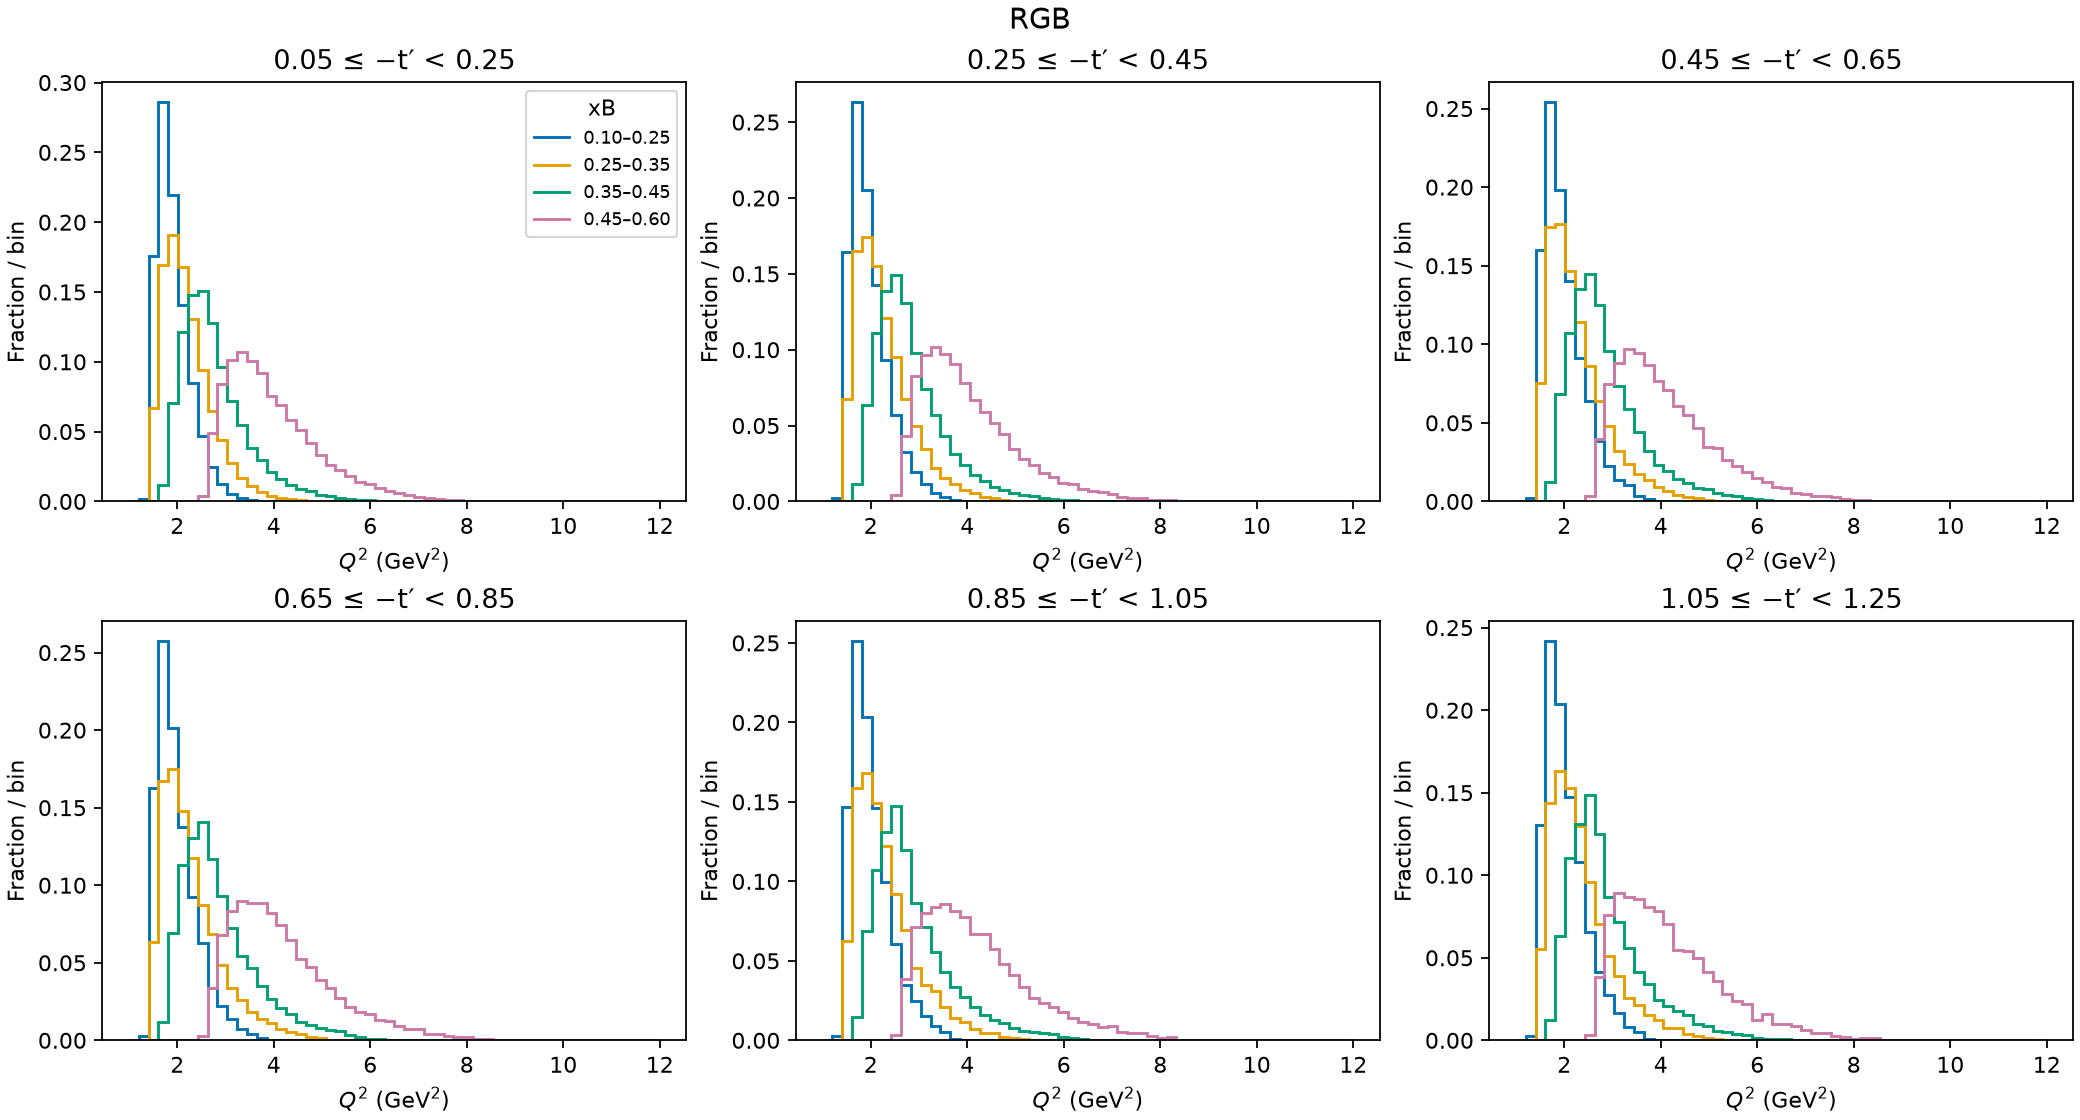
\includegraphics[width=0.98\linewidth]{figures/channel_selection/kinematic_distributions/RGB/05_Q2_by_analysis_bin.png}
\caption{RGB D$_2$: $Q^2$ distributions in the 24 $(x_B,-t^\prime)$ bins. Each panel selects one $-t^\prime$ interval, and colors distinguish the four $x_B$ intervals.}
\label{fig:eppi_kin_rgb_Q2}
\end{figure}

\begin{figure}[p]
\centering
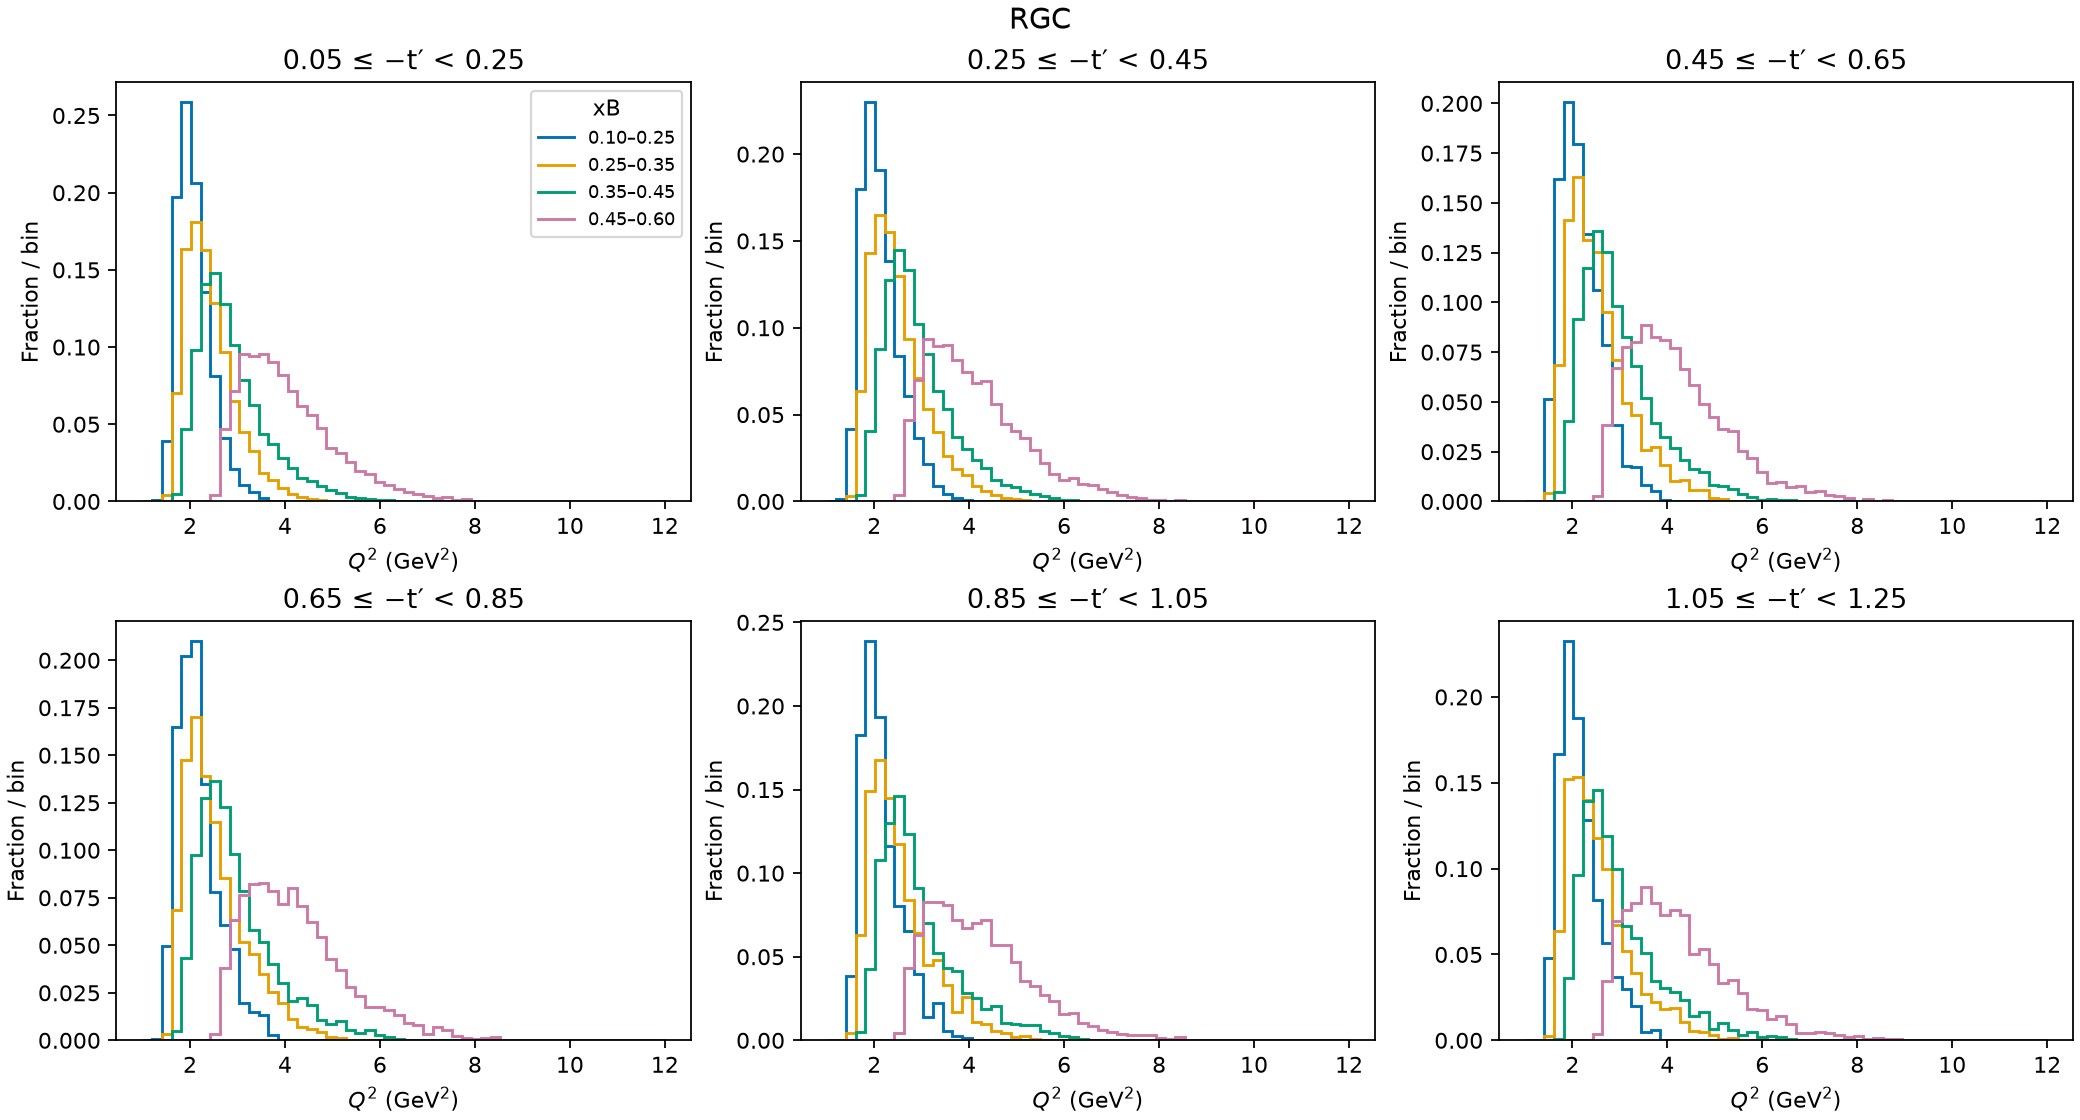
\includegraphics[width=0.98\linewidth]{figures/channel_selection/kinematic_distributions/RGC/05_Q2_by_analysis_bin.png}
\caption{RGC ND$_3$: $Q^2$ distributions in the 24 $(x_B,-t^\prime)$ bins. Each panel selects one $-t^\prime$ interval, and colors distinguish the four $x_B$ intervals.}
\label{fig:eppi_kin_rgc_Q2}
\end{figure}
\clearpage

% \begin{figure}[p]
% \centering
% 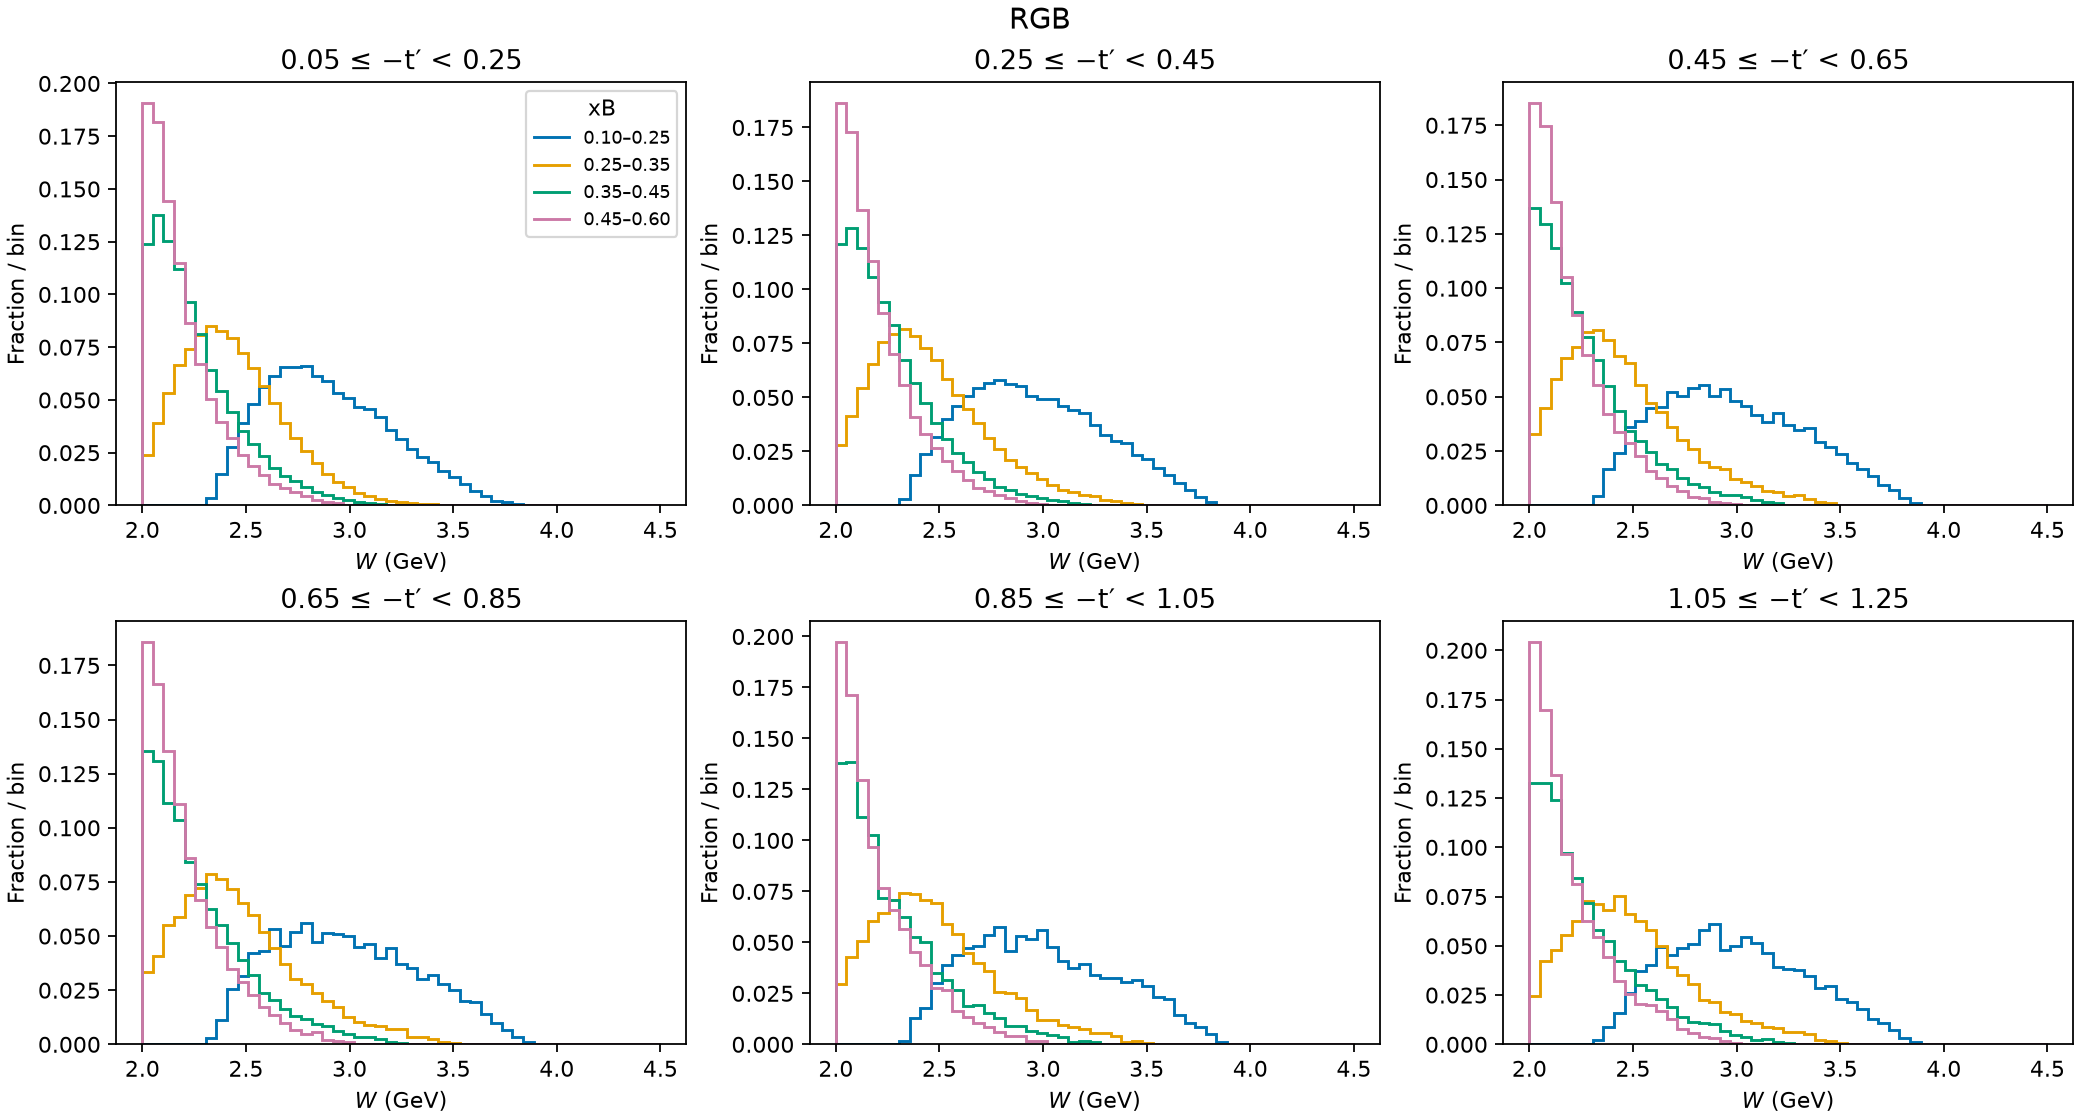
\includegraphics[width=0.98\linewidth]{figures/channel_selection/kinematic_distributions/RGB/06_W_by_analysis_bin.png}
% \caption{RGB D$_2$: $W$ distributions in the 24 $(x_B,-t^\prime)$ bins. Each panel selects one $-t^\prime$ interval, and colors distinguish the four $x_B$ intervals.}
% \label{fig:eppi_kin_rgb_W}
% \end{figure}

% \begin{figure}[p]
% \centering
% 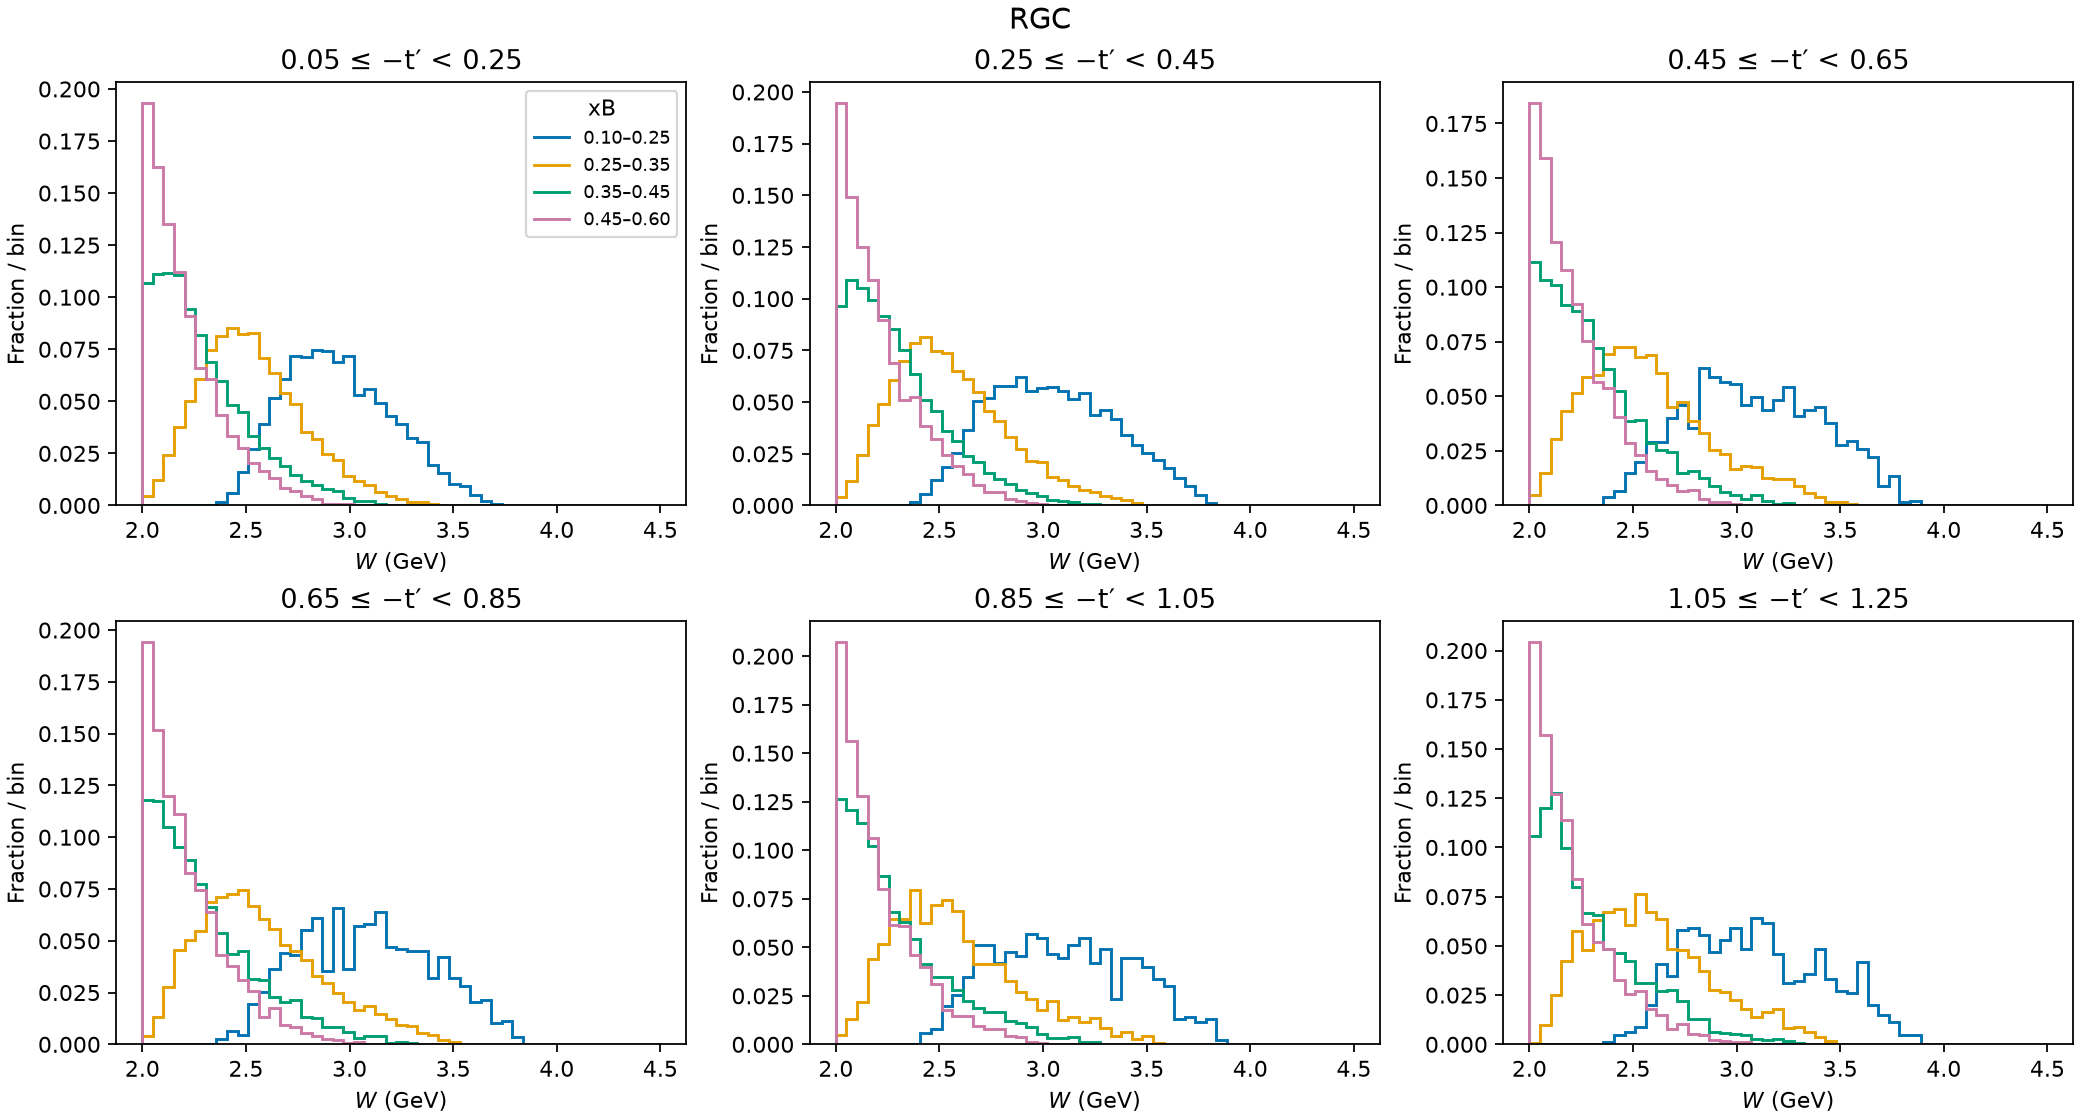
\includegraphics[width=0.98\linewidth]{figures/channel_selection/kinematic_distributions/RGC/06_W_by_analysis_bin.png}
% \caption{RGC ND$_3$: $W$ distributions in the 24 $(x_B,-t^\prime)$ bins. Each panel selects one $-t^\prime$ interval, and colors distinguish the four $x_B$ intervals. }
% \label{fig:eppi_kin_rgc_W}
% \end{figure}
% \clearpage

% \begin{figure}[p]
% \centering
% 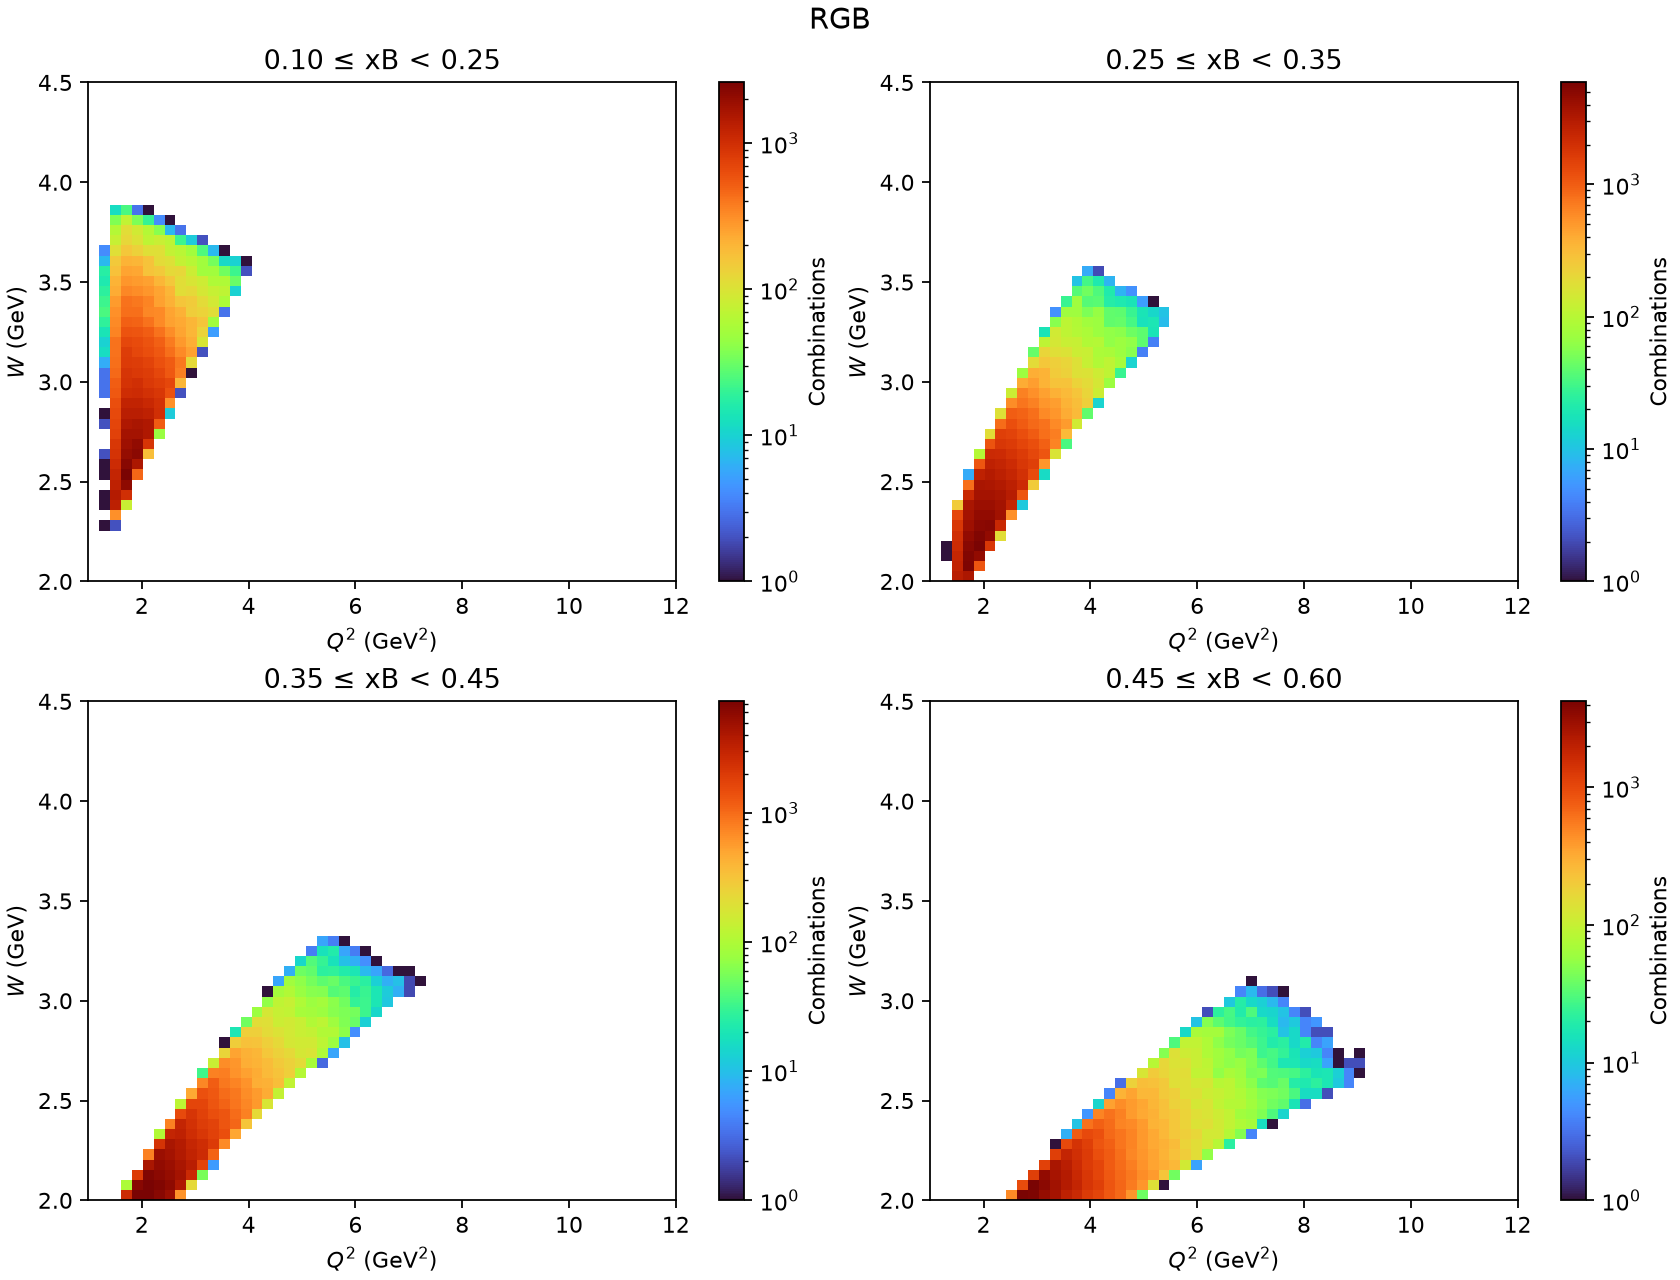
\includegraphics[width=0.98\linewidth]{figures/channel_selection/kinematic_distributions/RGB/07_Q2_W_by_xB.png}
% \caption{RGB D$_2$: $Q^2$--$W$ coverage in the four analysis $x_B$ intervals. }
% \label{fig:eppi_kin_rgb_Q2_W}
% \end{figure}

% \begin{figure}[p]
% \centering
% 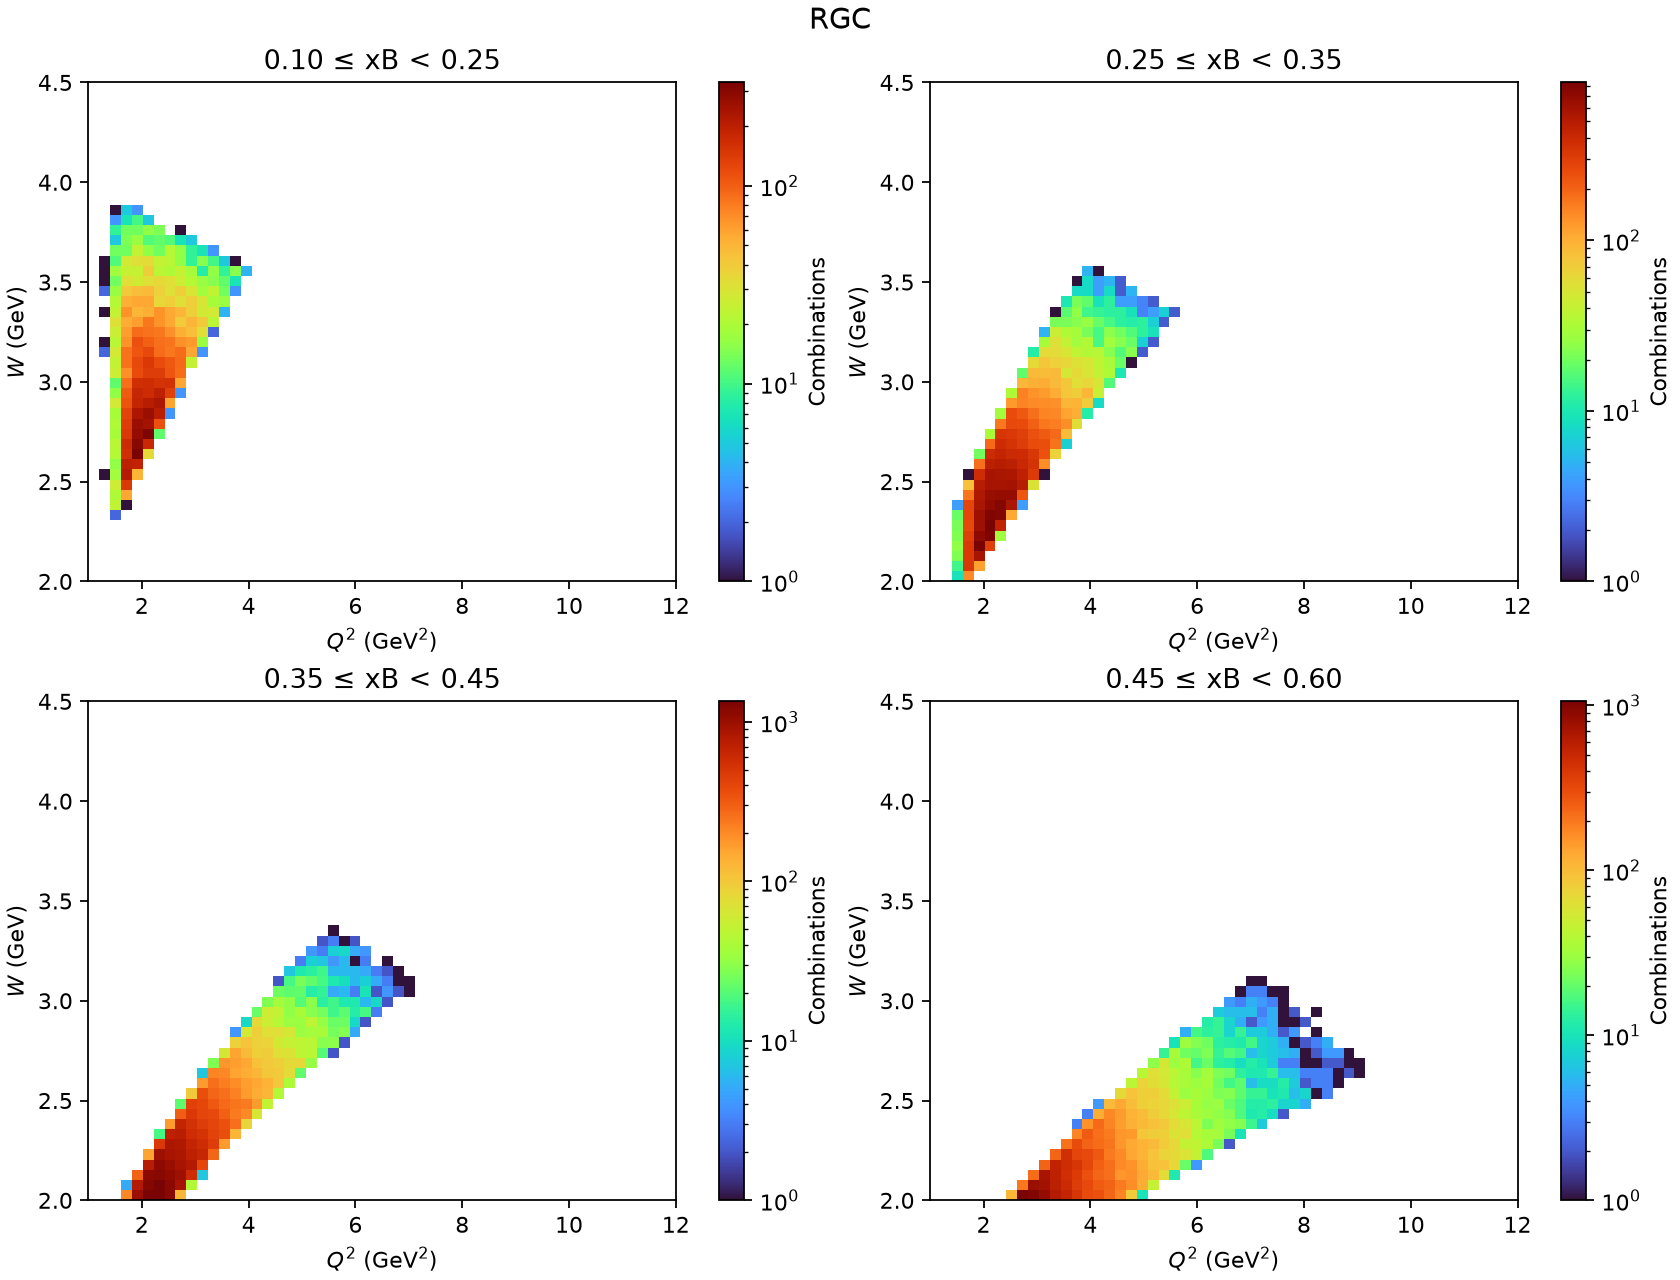
\includegraphics[width=0.98\linewidth]{figures/channel_selection/kinematic_distributions/RGC/07_Q2_W_by_xB.png}
% \caption{RGC ND$_3$: $Q^2$--$W$ coverage in the four analysis $x_B$ intervals. }
% \label{fig:eppi_kin_rgc_Q2_W}
% \end{figure}
% \clearpage

\begin{figure}[p]
\centering
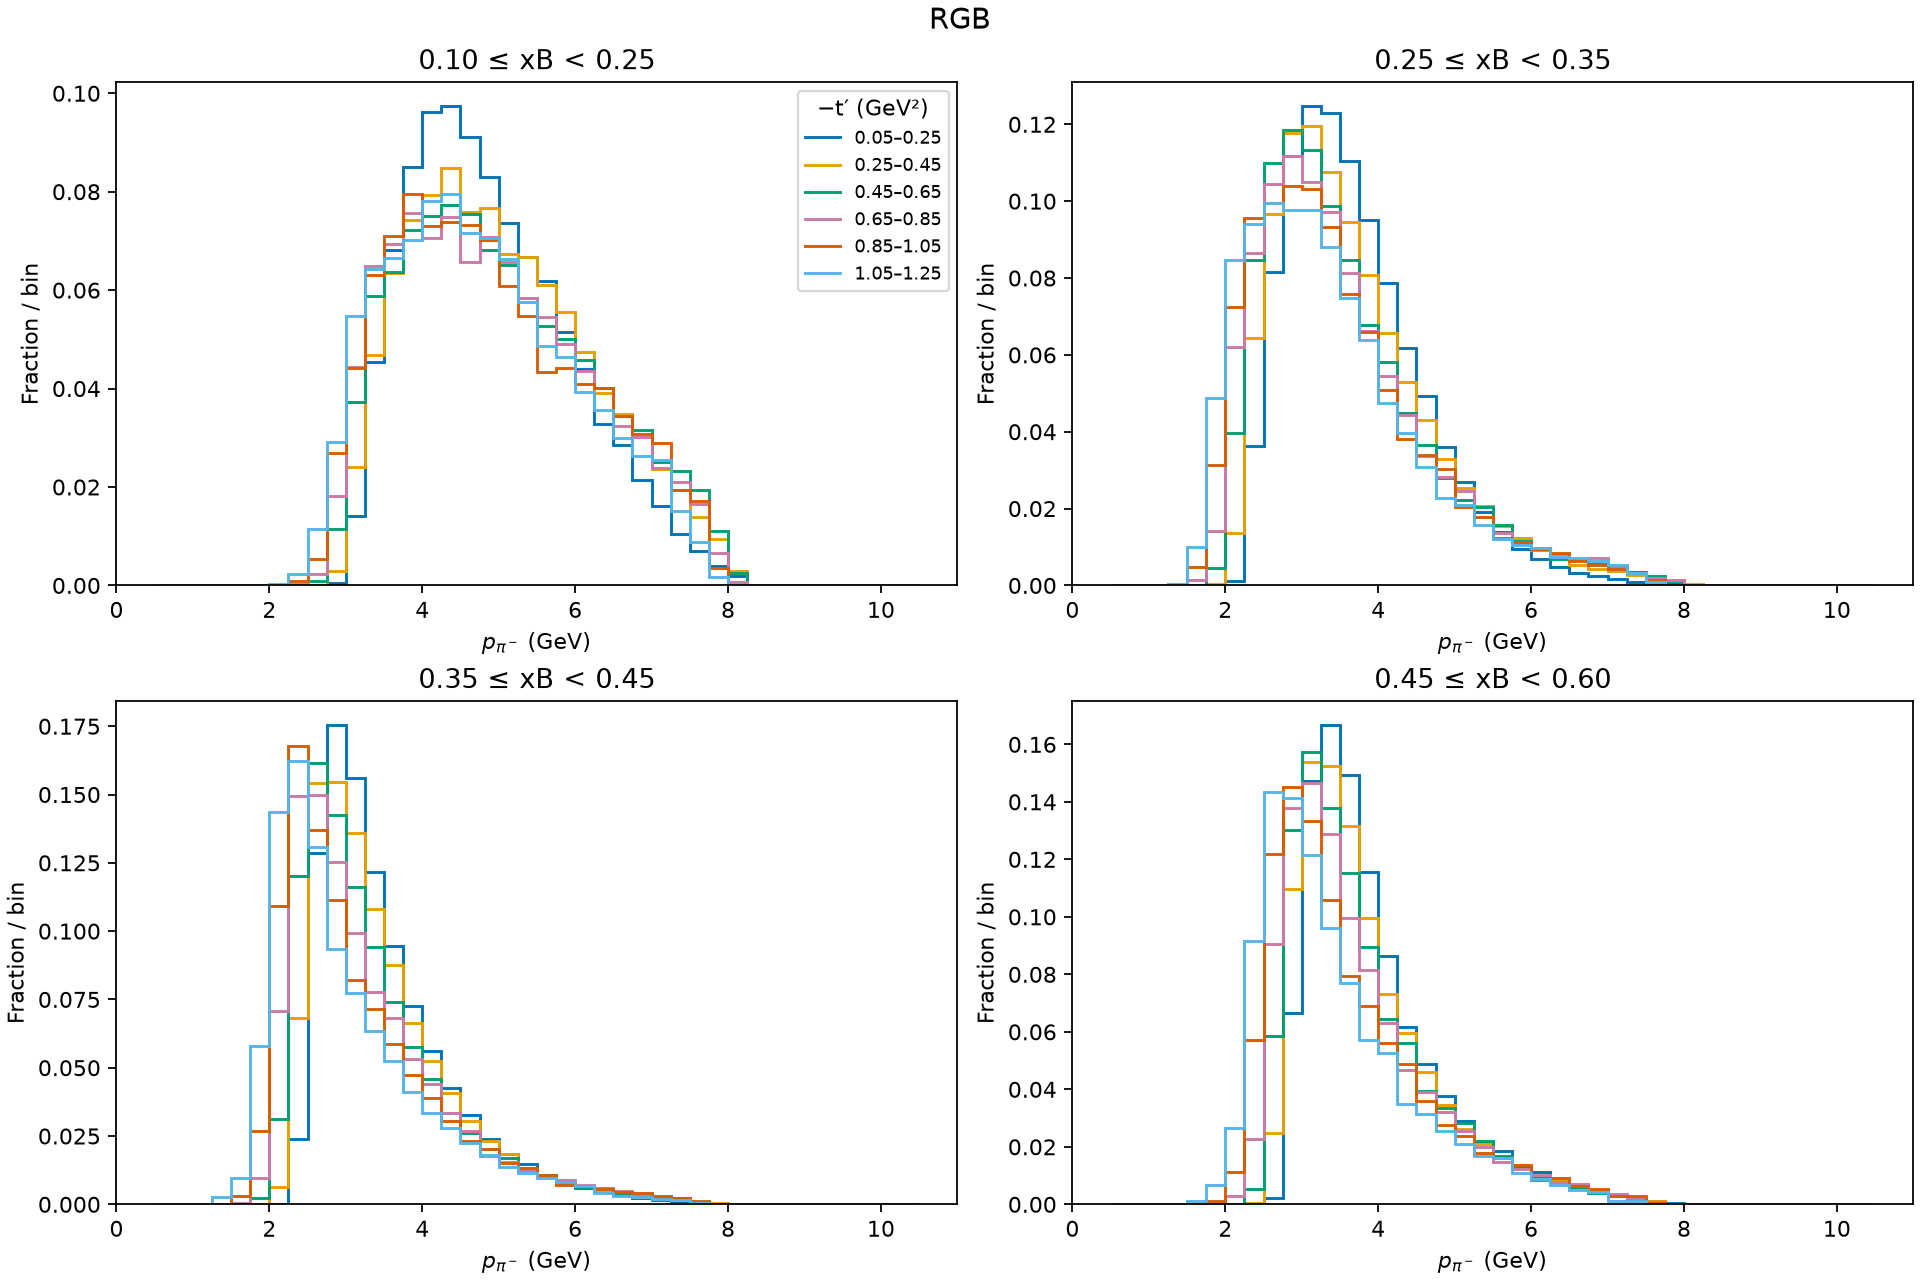
\includegraphics[width=0.98\linewidth]{figures/channel_selection/kinematic_distributions/RGB/08_pion_momentum_by_analysis_bin.png}
\caption{RGB D$_2$: Detected $\pi^-$ momentum distributions in all 24 analysis bins. Each panel selects an $x_B$ interval, and the six colors distinguish the $-t^\prime$ intervals. }
\label{fig:eppi_kin_rgb_pion}
\end{figure}

\begin{figure}[p]
\centering
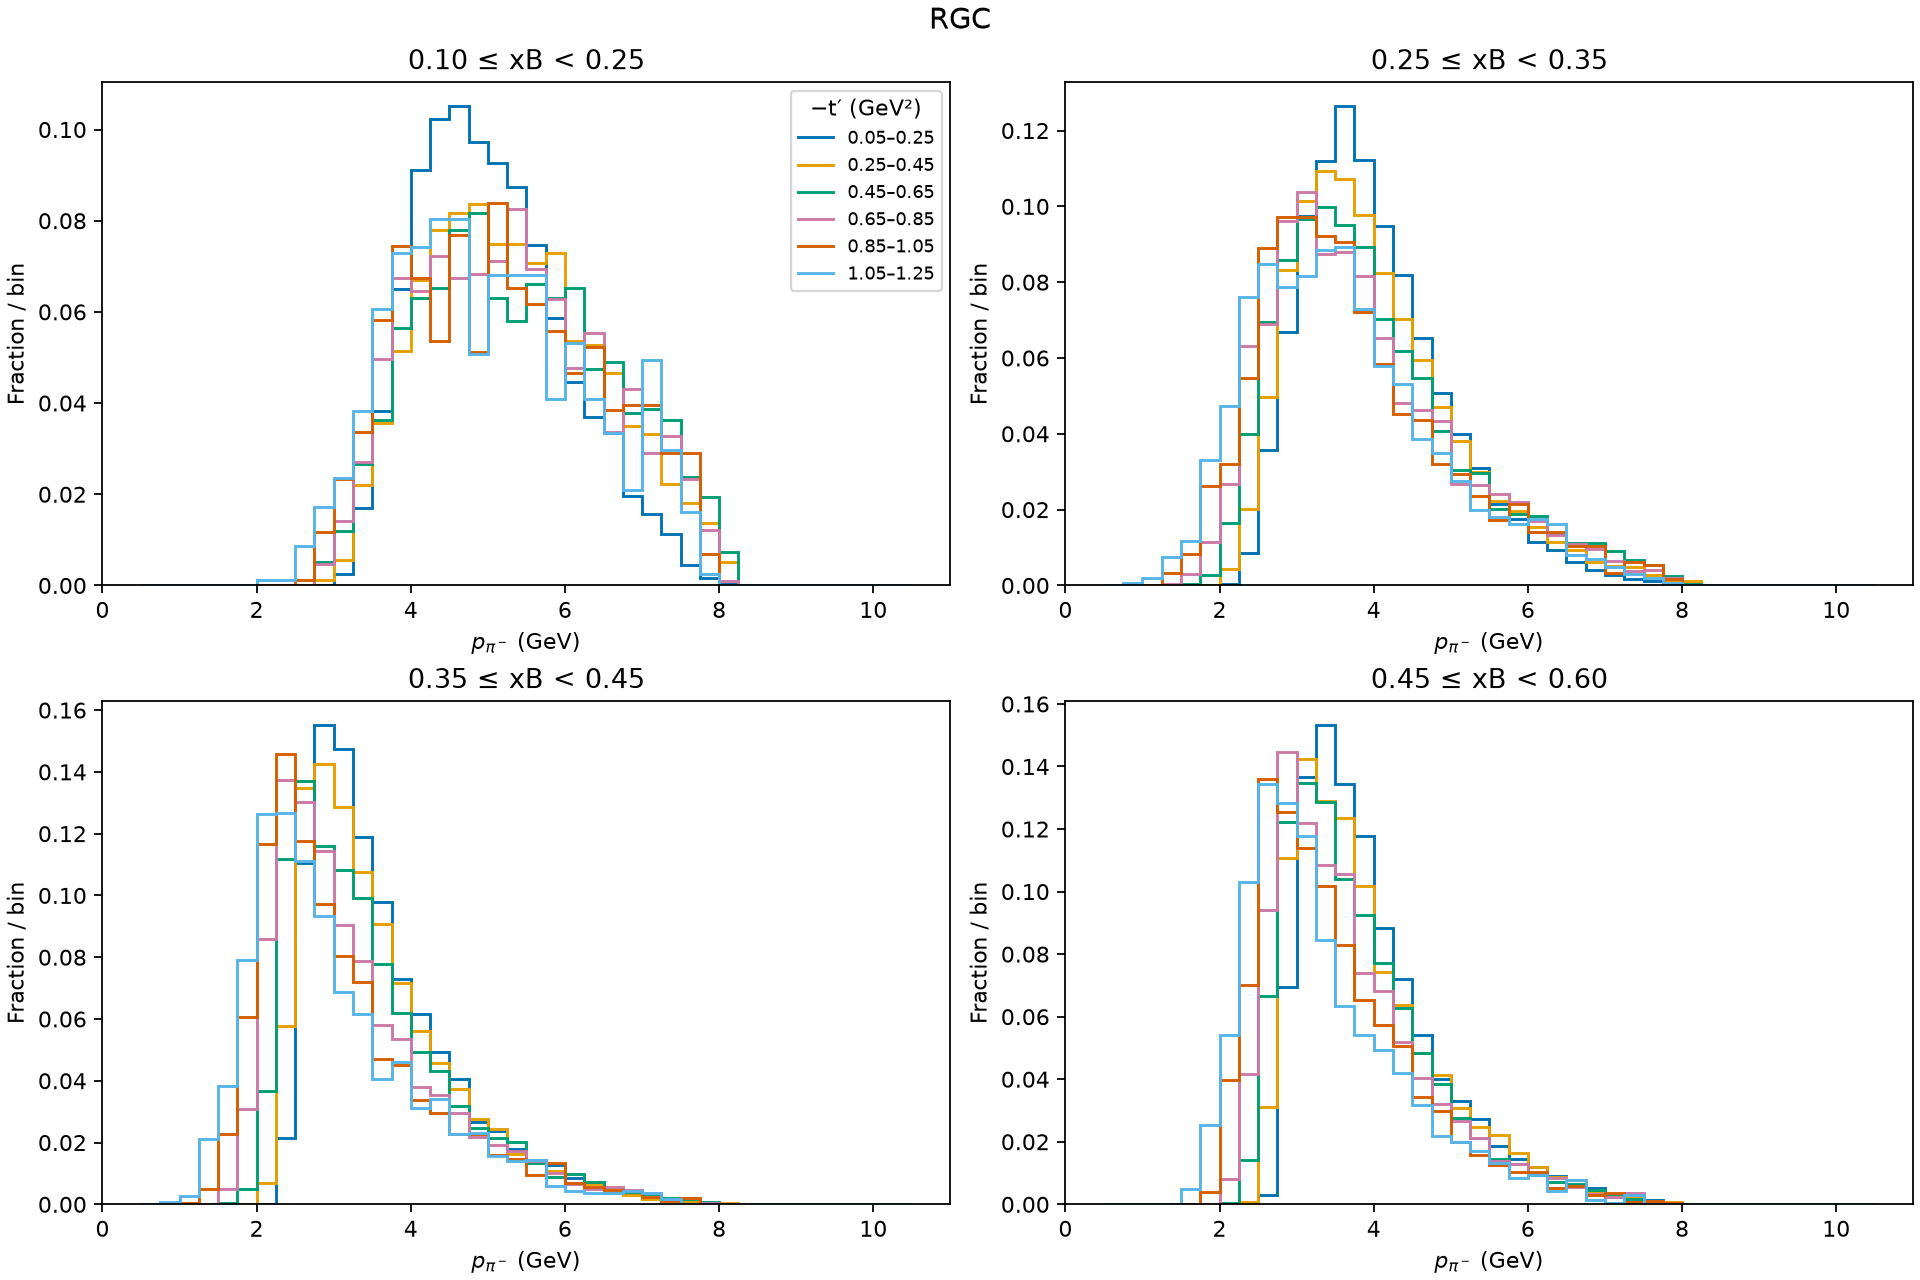
\includegraphics[width=0.98\linewidth]{figures/channel_selection/kinematic_distributions/RGC/08_pion_momentum_by_analysis_bin.png}
\caption{RGC ND$_3$: Detected $\pi^-$ momentum distributions in all 24 analysis bins. Each panel selects an $x_B$ interval, and the six colors distinguish the $-t^\prime$ intervals. }
\label{fig:eppi_kin_rgc_pion}
\end{figure}
\clearpage

\begin{figure}[p]
\centering
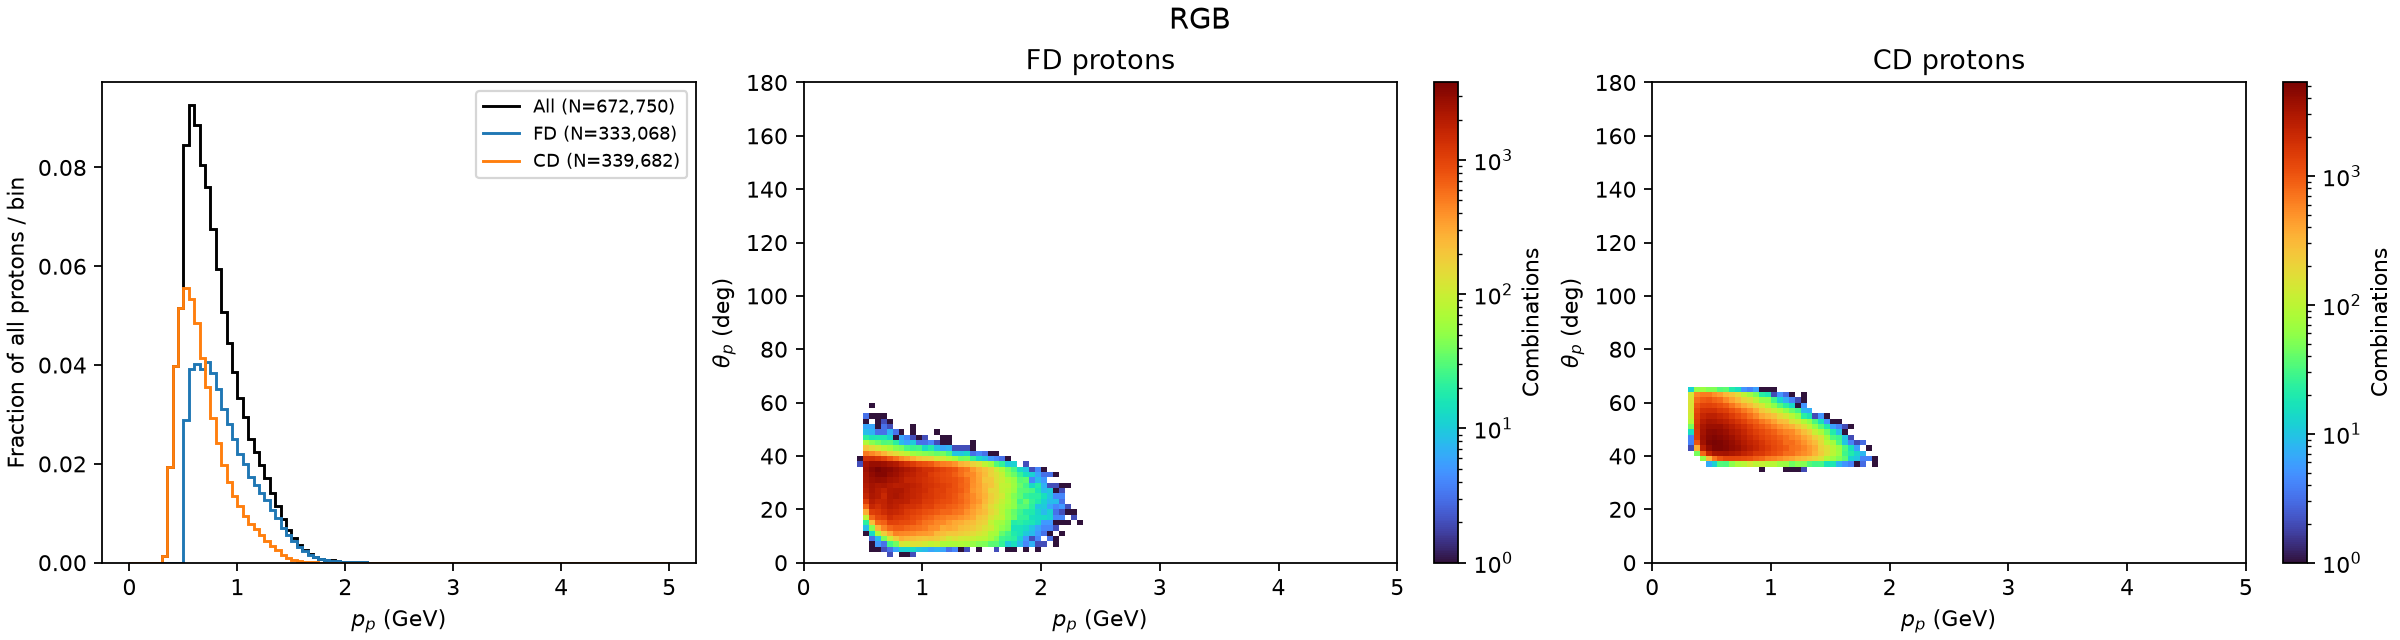
\includegraphics[width=0.99\linewidth]{figures/channel_selection/kinematic_distributions/RGB/09_proton_momentum_FD_CD.png}
\caption{RGB D$_2$: Detected-proton momentum and angular coverage. The left panel shows all protons (black), FD protons (blue) and CD protons (orange), with a common normalization to the full selected proton population. The middle and right panels show the FD and CD momentum--polar-angle distributions separately.}
\label{fig:eppi_kin_rgb_proton}
\end{figure}

\begin{figure}[p]
\centering
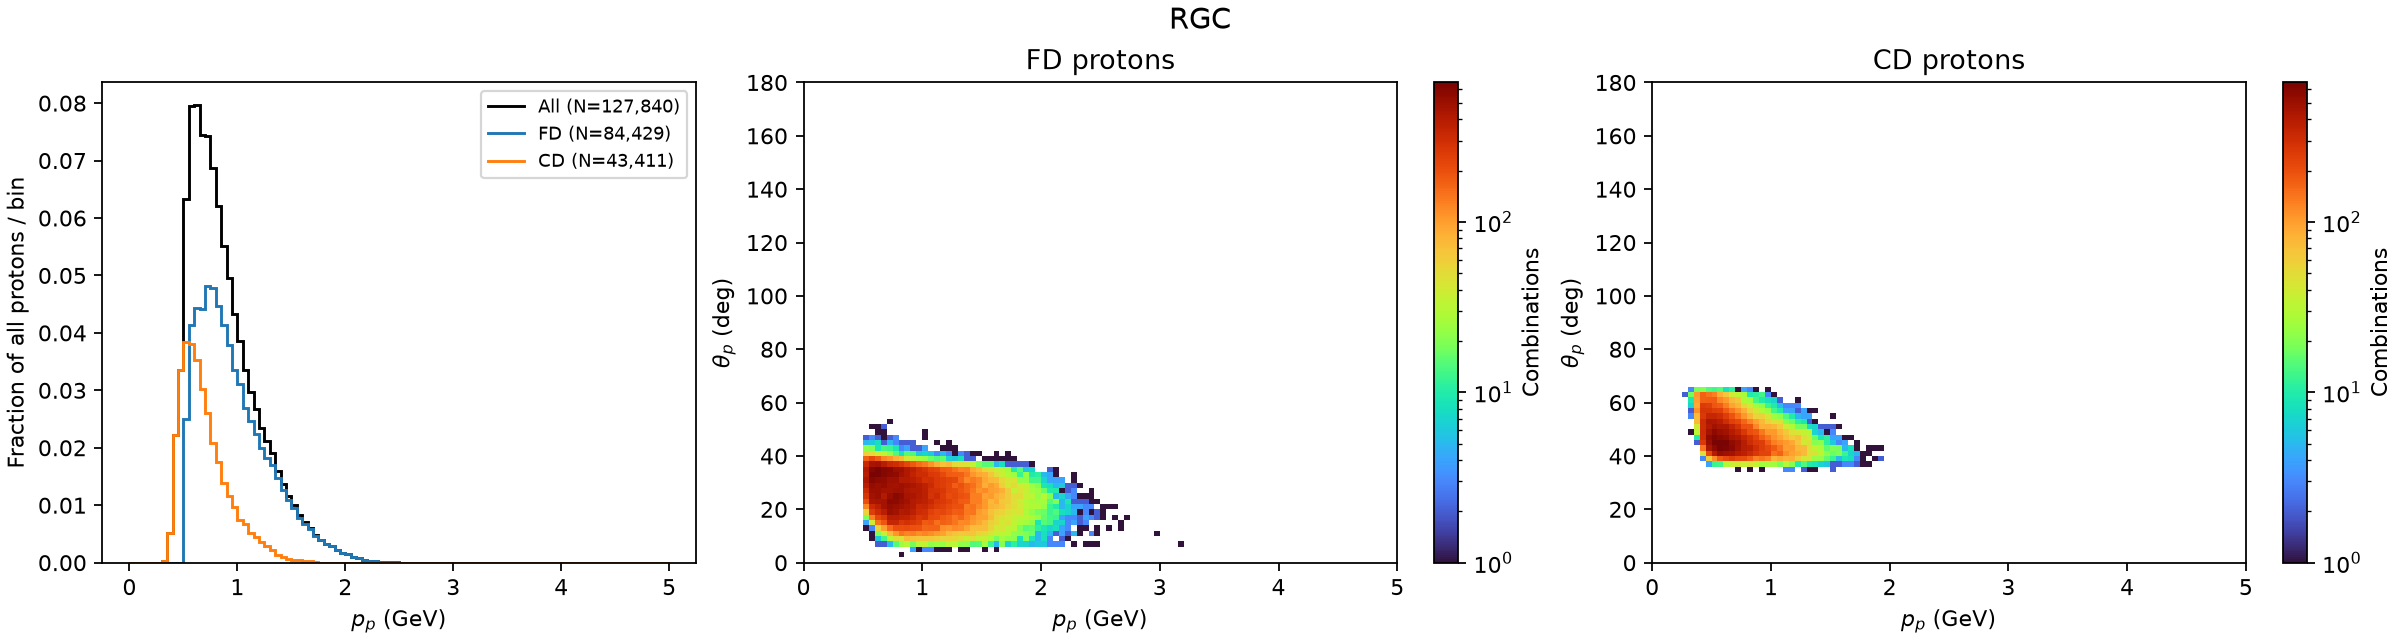
\includegraphics[width=0.99\linewidth]{figures/channel_selection/kinematic_distributions/RGC/09_proton_momentum_FD_CD.png}
\caption{RGC ND$_3$: Detected-proton momentum and angular coverage. The left panel shows all protons (black), FD protons (blue) and CD protons (orange), with a common normalization to the full selected proton population. The middle and right panels show the FD and CD momentum--polar-angle distributions separately.}
\label{fig:eppi_kin_rgc_proton}
\end{figure}
\clearpage
\begin{figure}[p]\centering
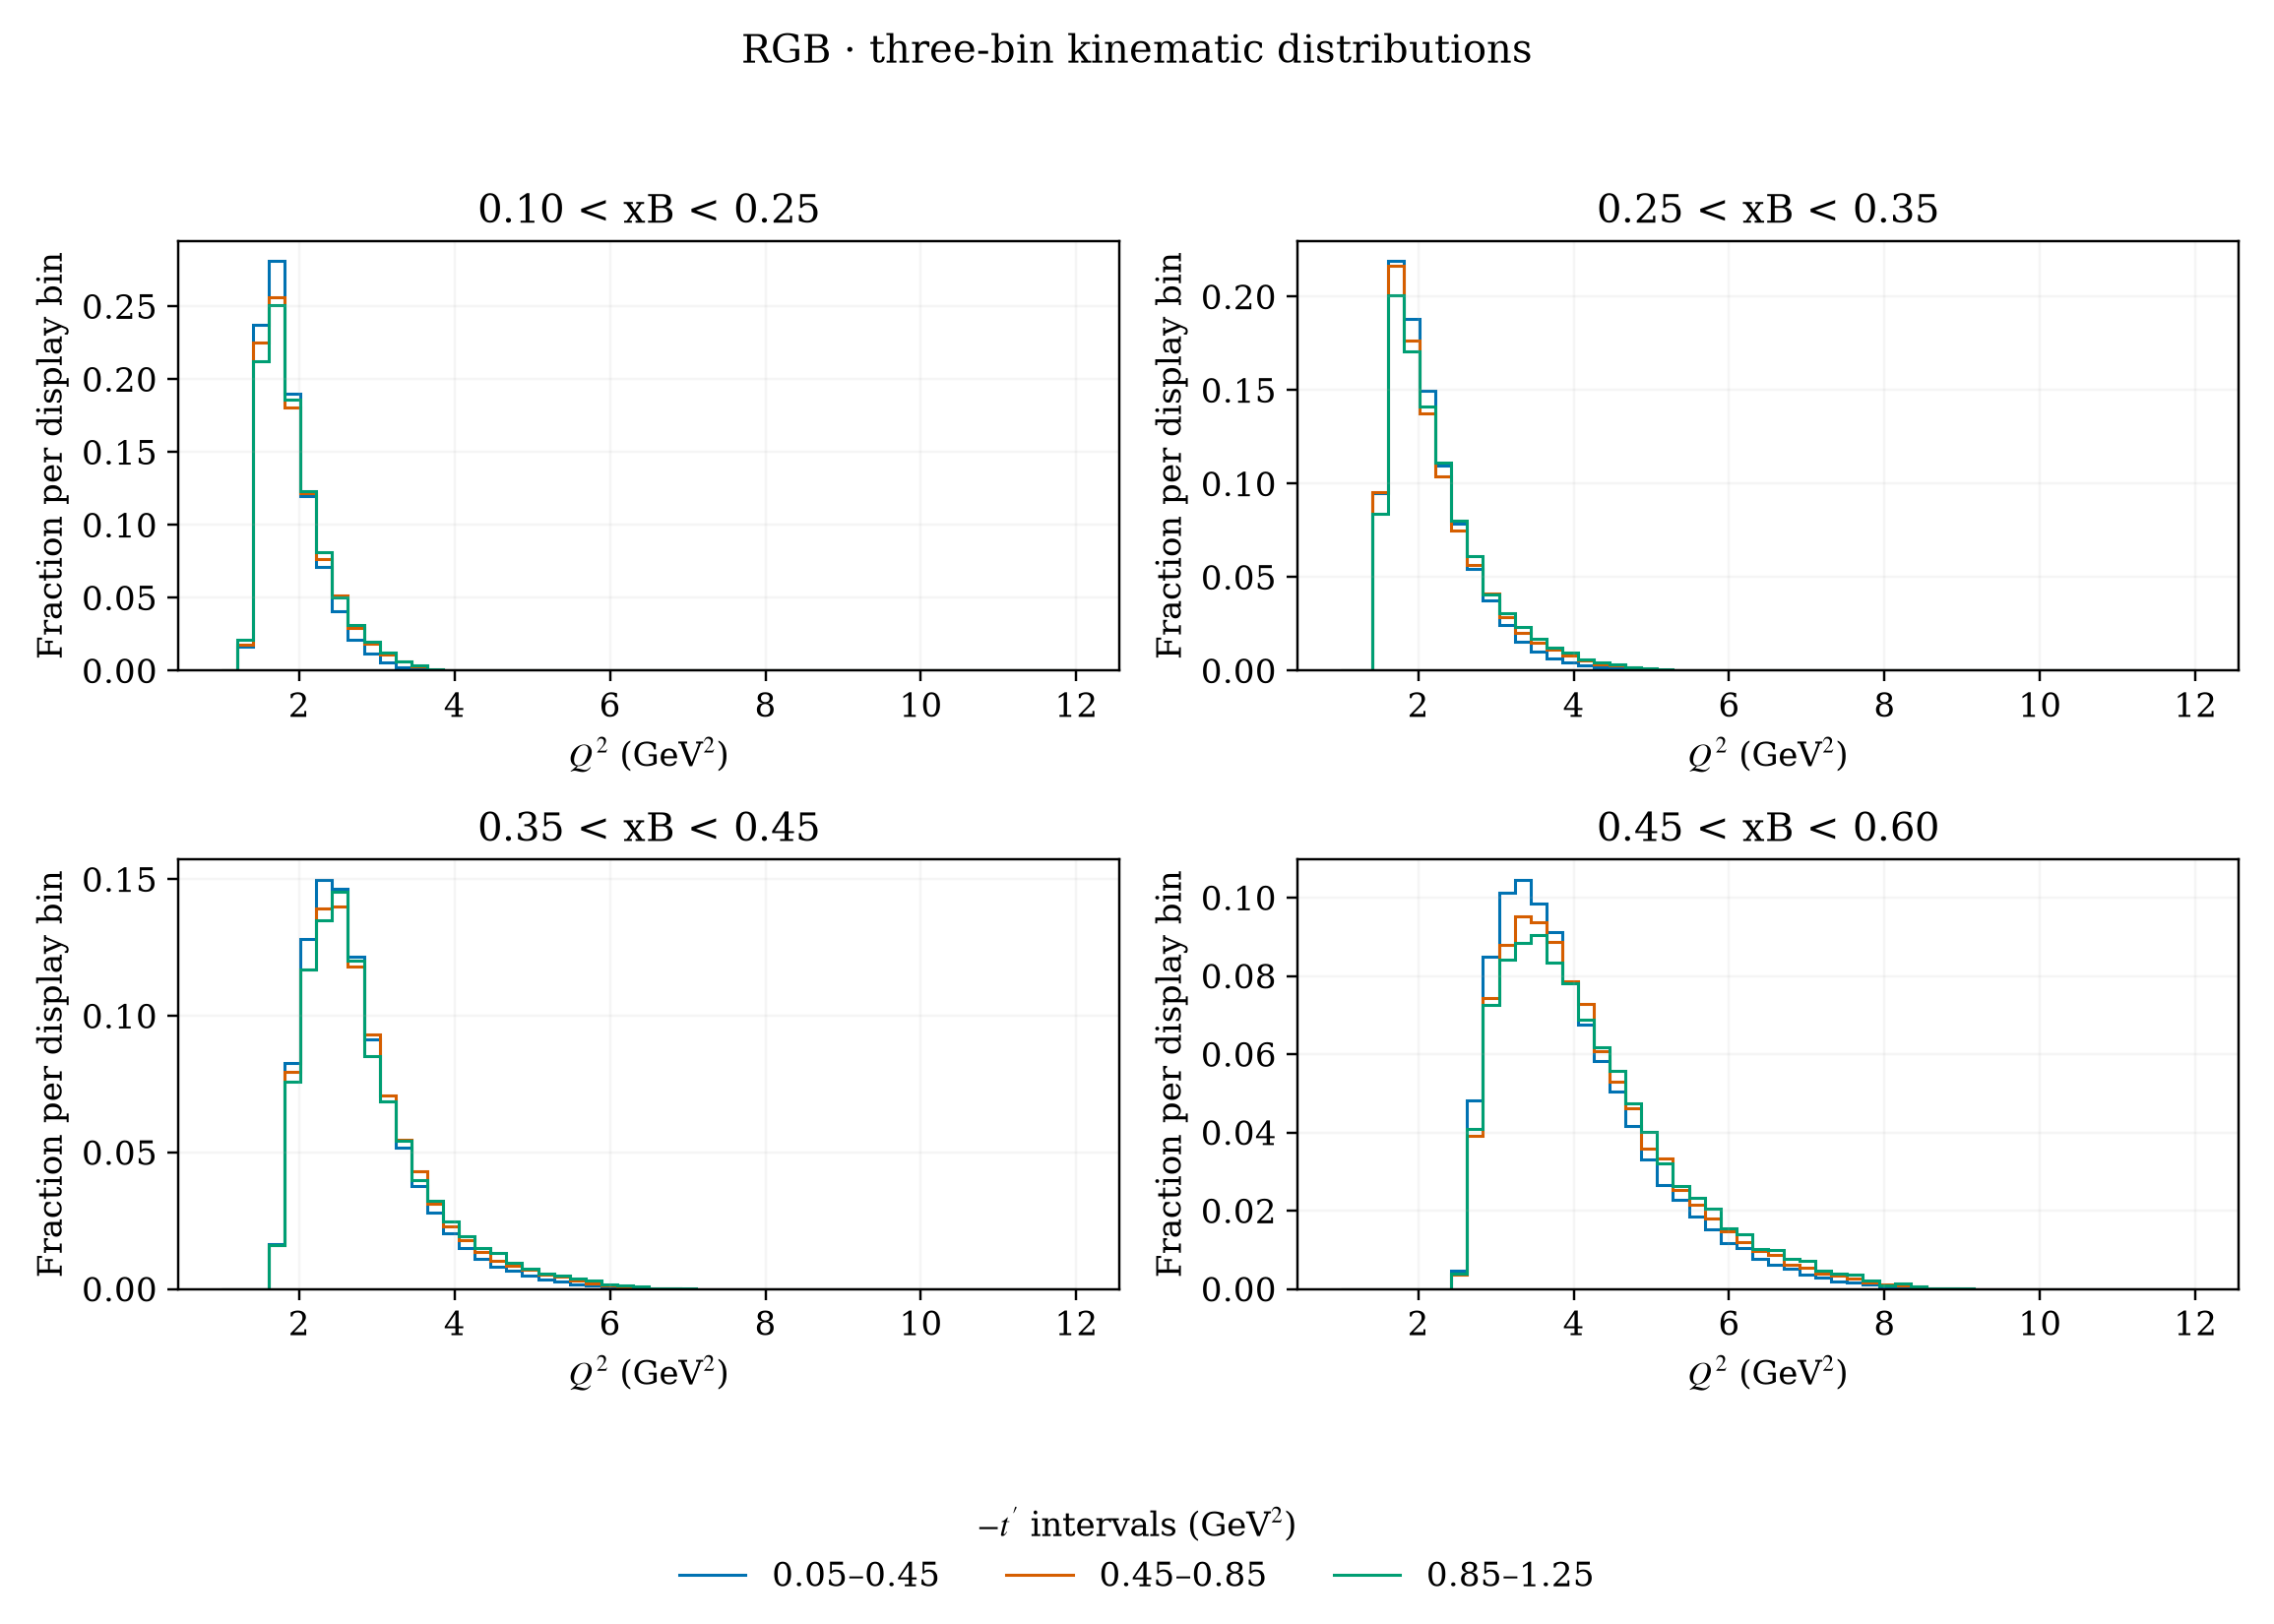
\includegraphics[width=\linewidth]{figures/results/RGB_Q2_three_bin_2x2.png}
\caption{RGB distributions in the three merged target-sector bins. Each curve is normalized over its displayed range. The legends give the $-t^\prime$ intervals in GeV$^2$.}\label{fig:release_kin_RGBQ2}
\end{figure}
\clearpage
\begin{figure}[p]\centering
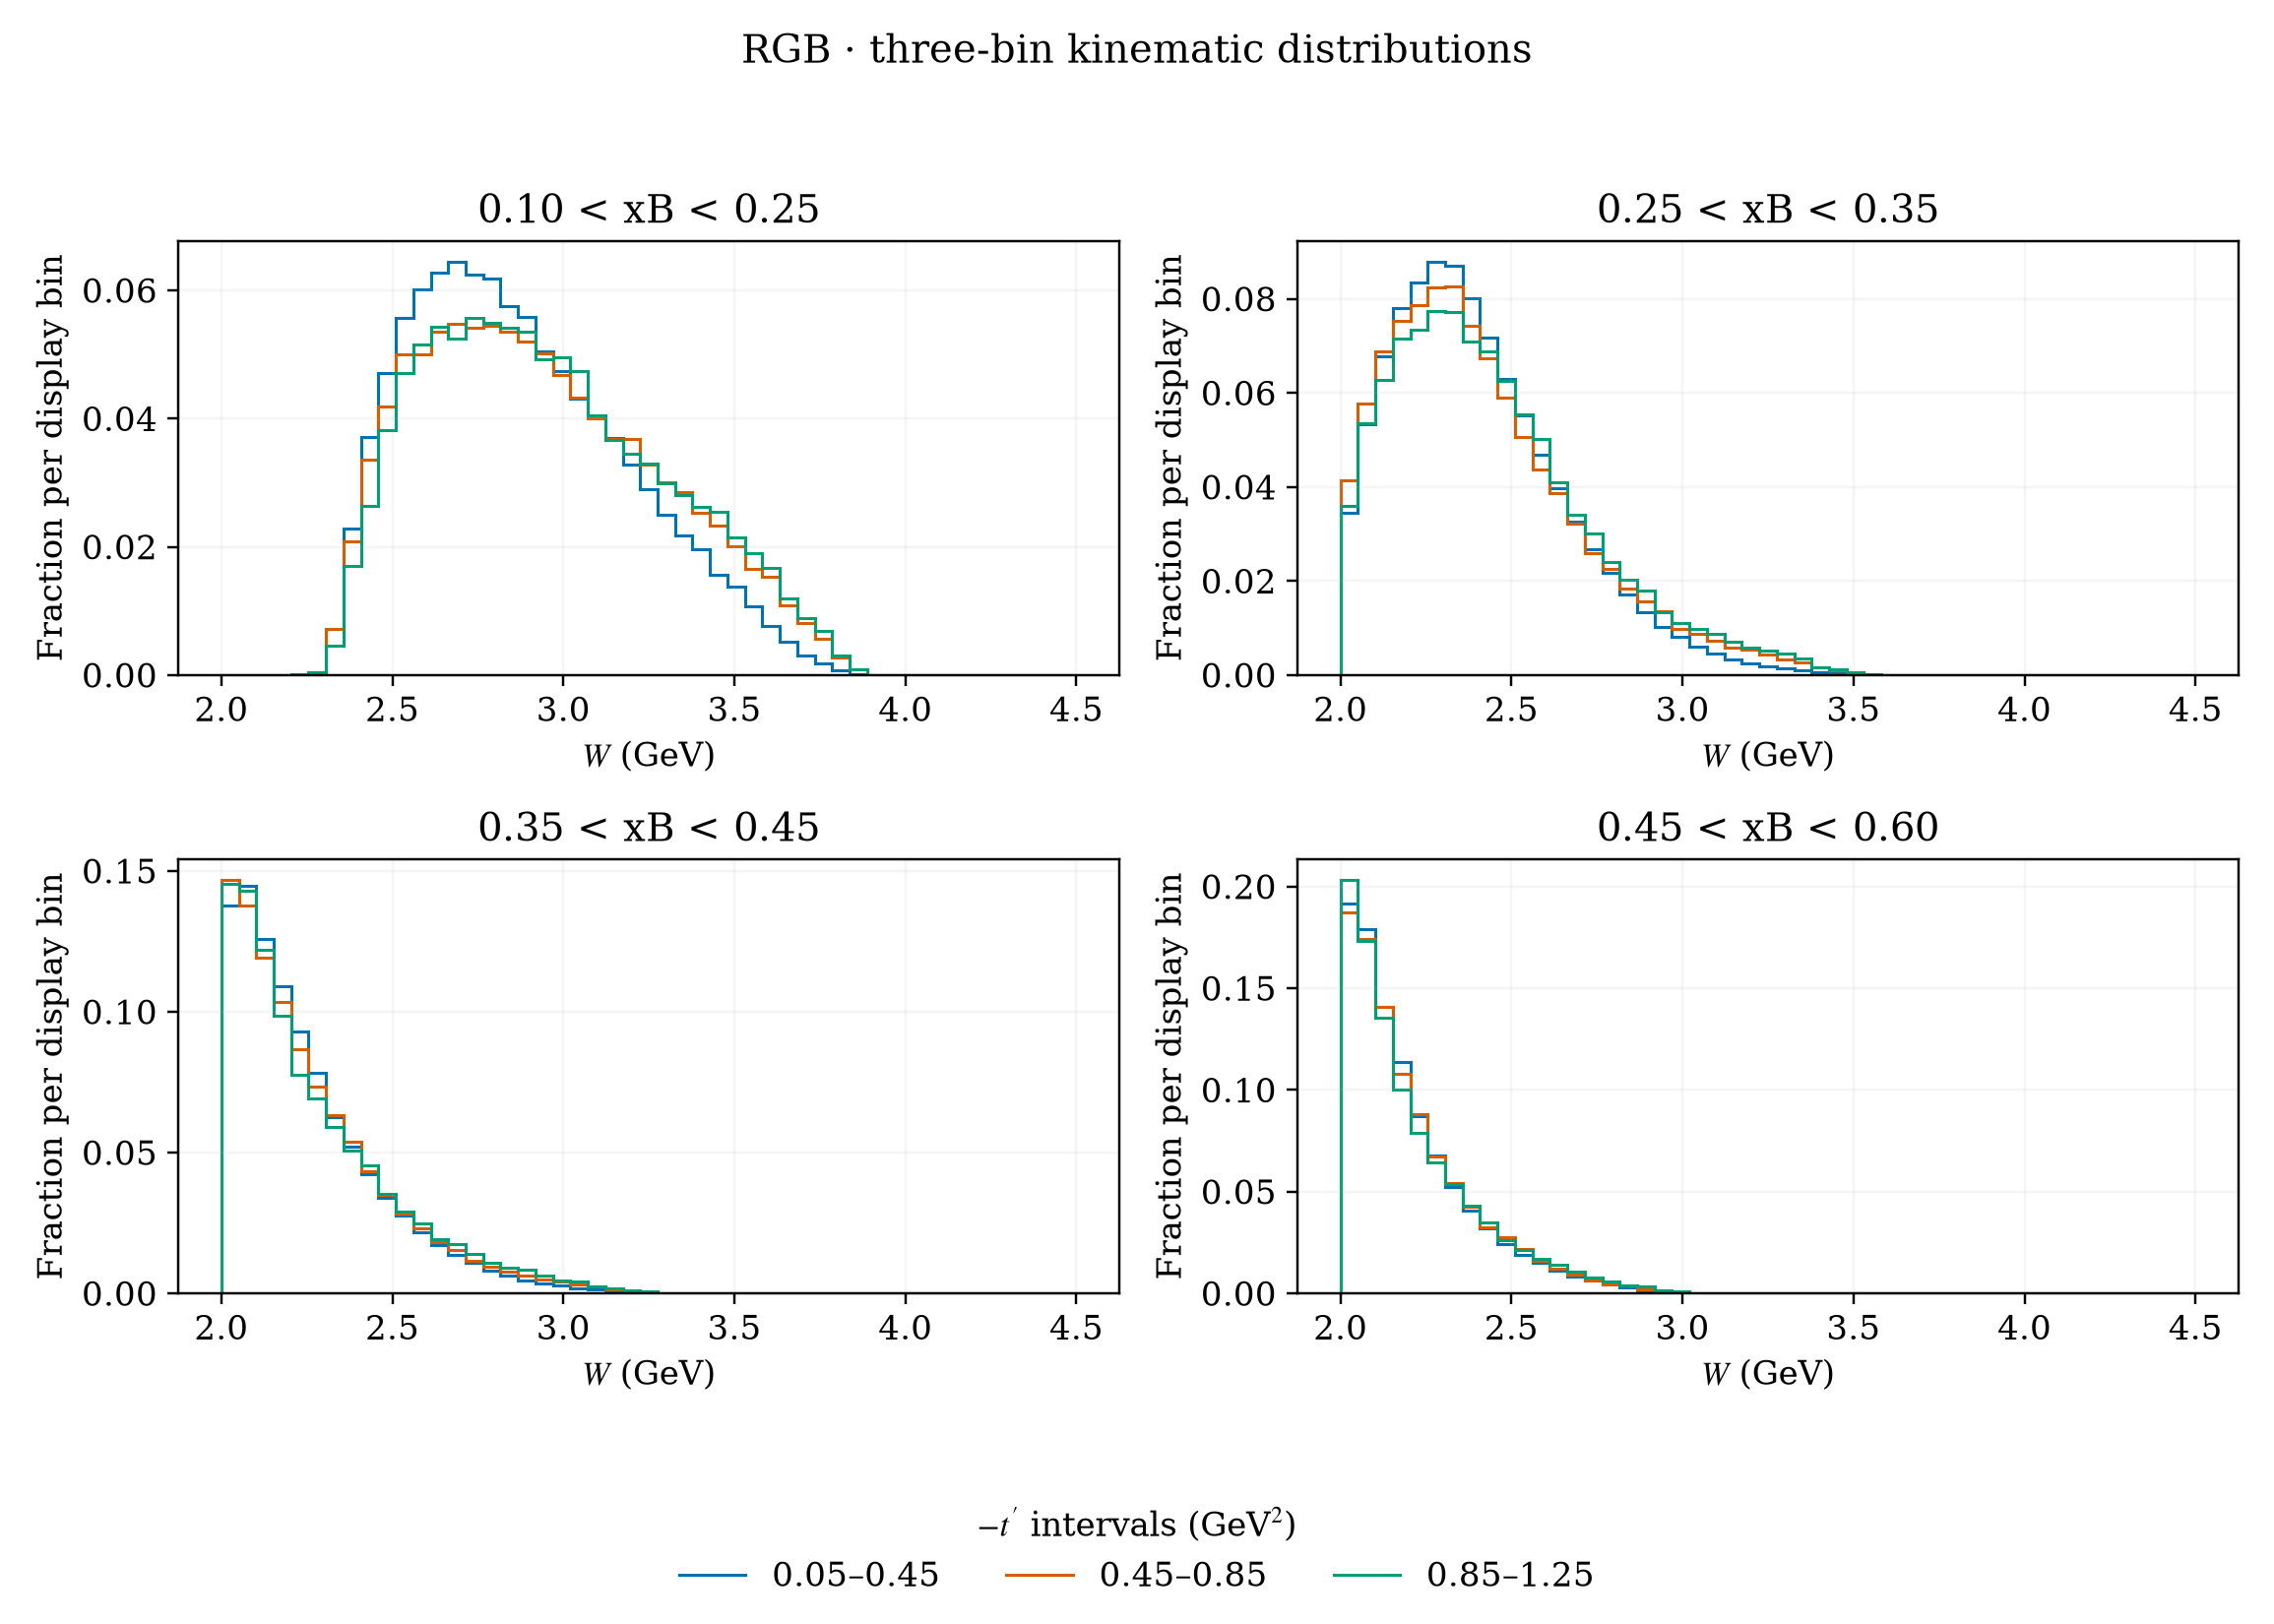
\includegraphics[width=\linewidth]{figures/results/RGB_W_three_bin_2x2.png}
\caption{RGB distributions in the three merged target-sector bins. Each curve is normalized over its displayed range. The legends give the $-t^\prime$ intervals in GeV$^2$.}\label{fig:release_kin_RGBW}
\end{figure}
\clearpage
\begin{figure}[p]\centering
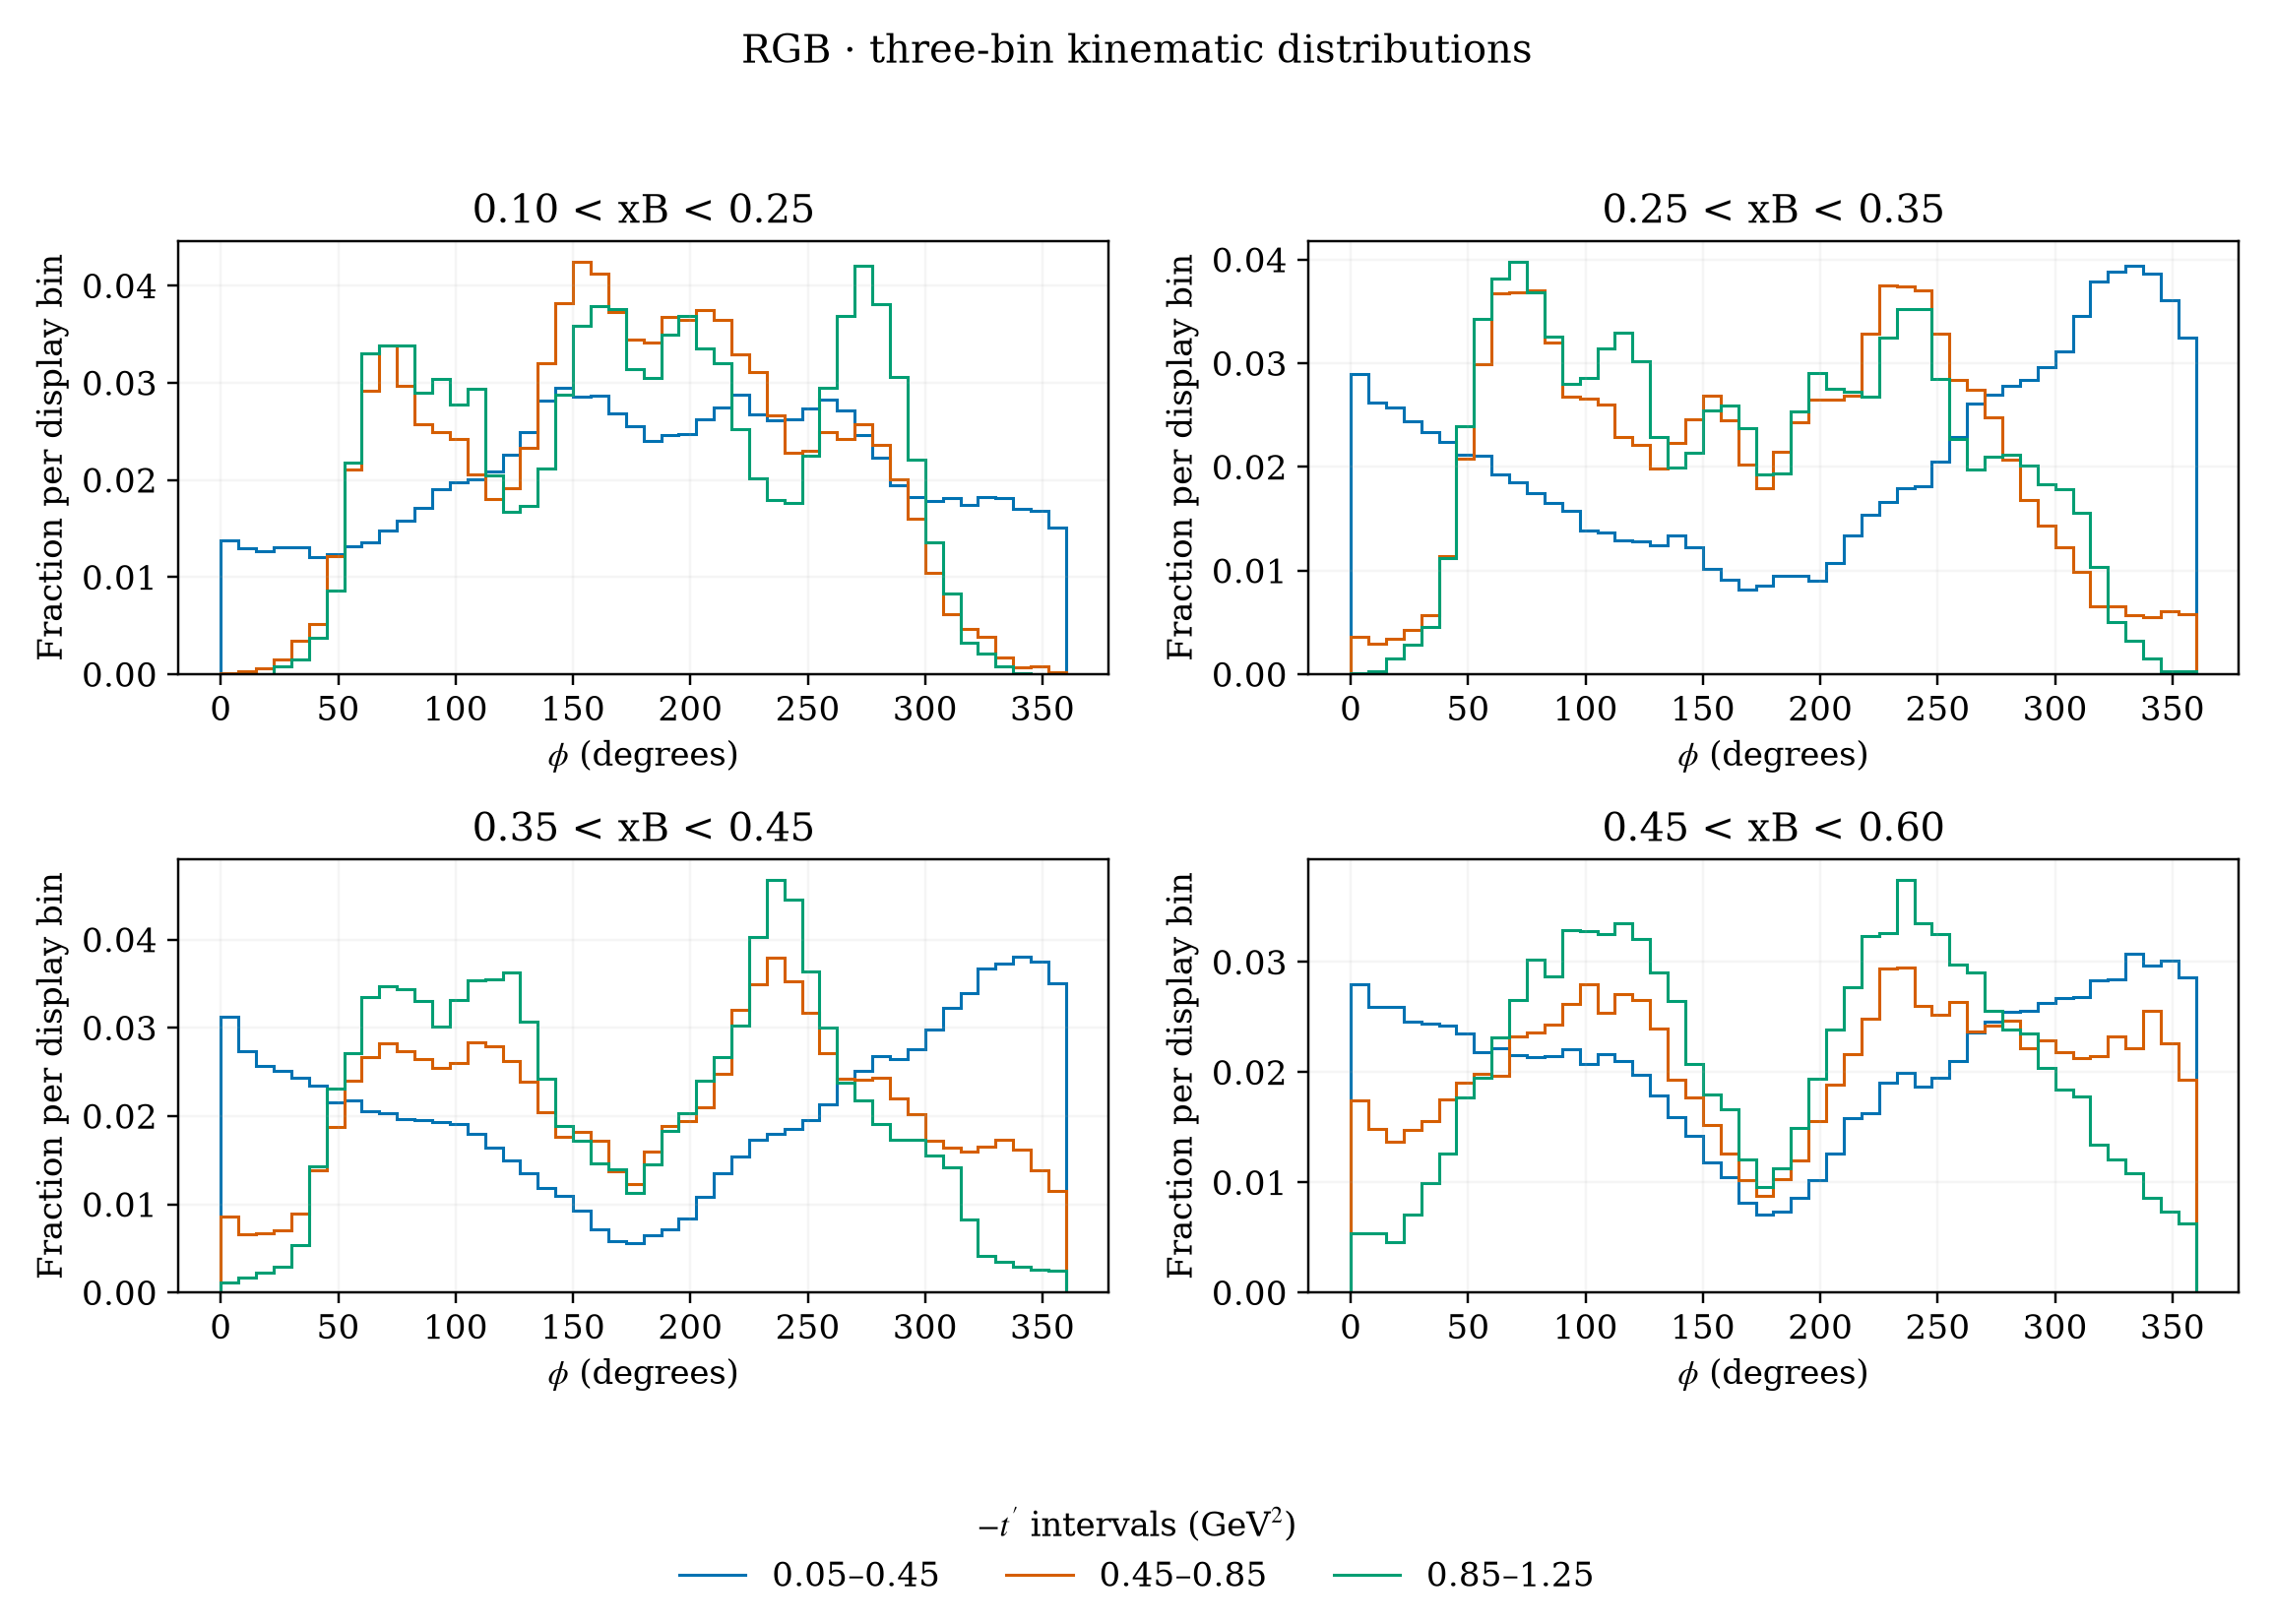
\includegraphics[width=\linewidth]{figures/results/RGB_phi_three_bin_2x2.png}
\caption{RGB distributions in the three merged target-sector bins. Each curve is normalized over its displayed range. The legends give the $-t^\prime$ intervals in GeV$^2$.}\label{fig:release_kin_RGBphi}
\end{figure}
\clearpage
\begin{figure}[p]\centering
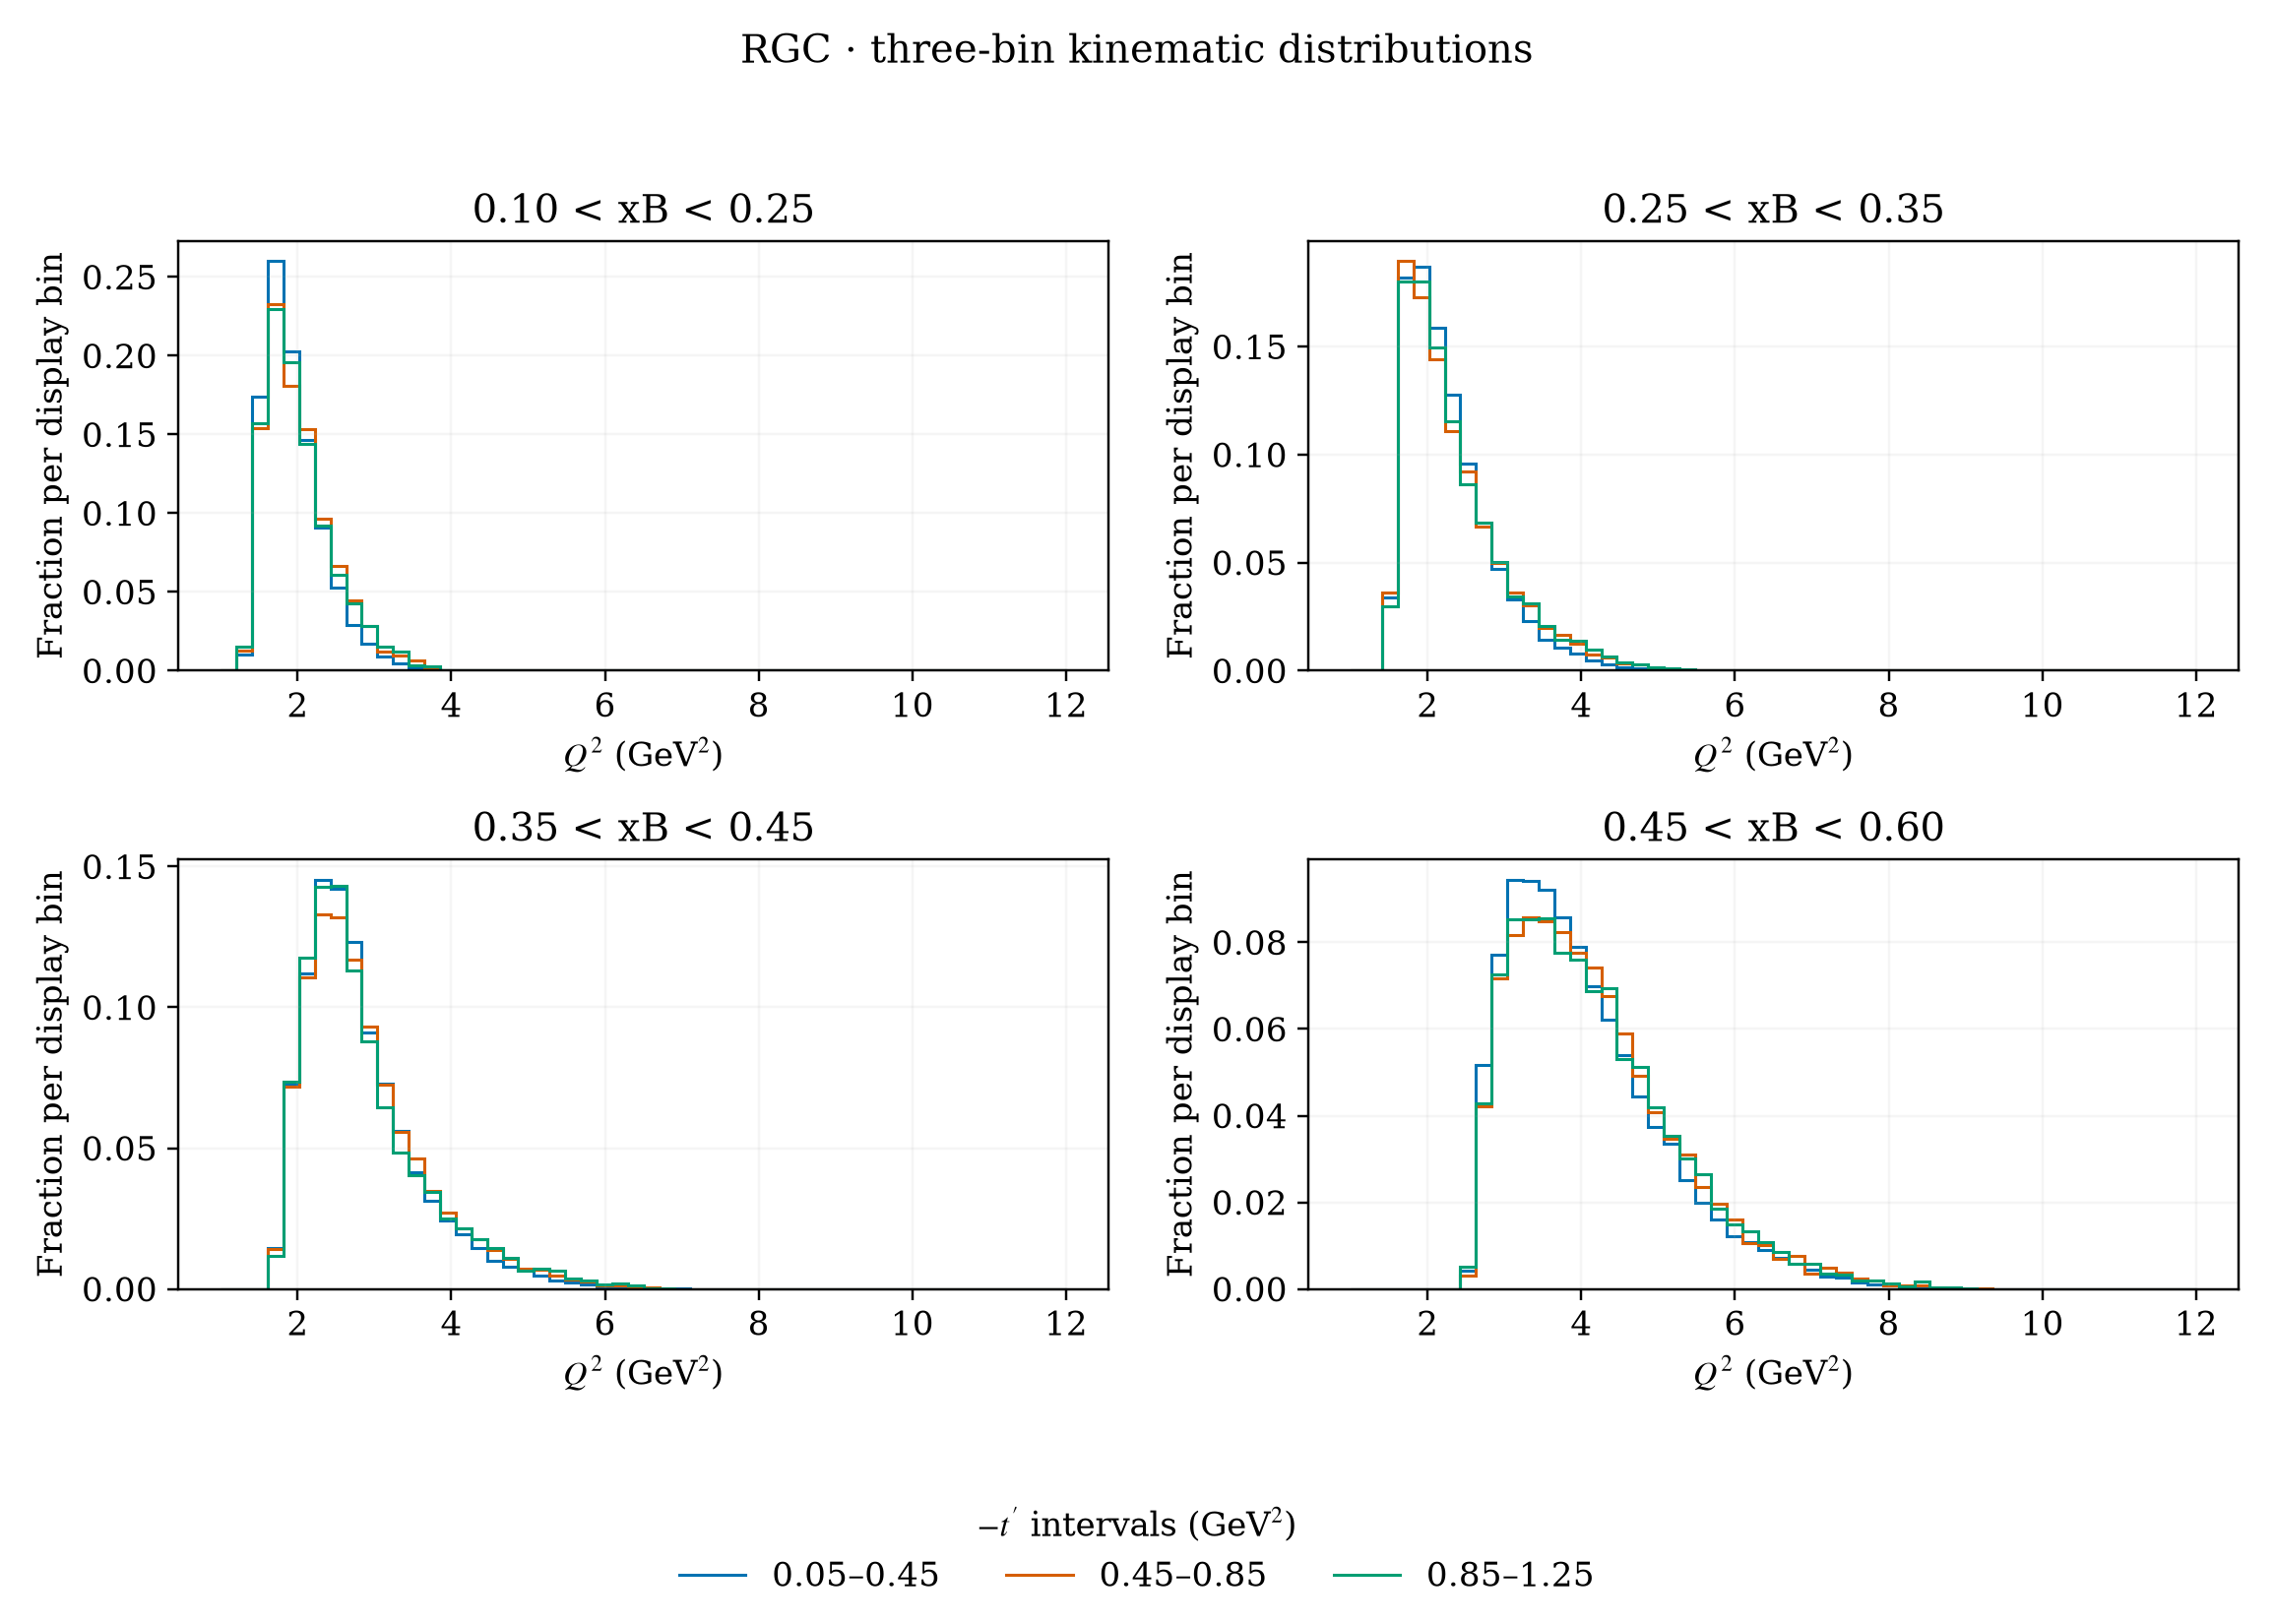
\includegraphics[width=\linewidth]{figures/results/RGC_Q2_three_bin_2x2.png}
\caption{RGC distributions in the three merged target-sector bins. Each curve is normalized over its displayed range. The legends give the $-t^\prime$ intervals in GeV$^2$.}\label{fig:release_kin_RGCQ2}
\end{figure}
\clearpage
\begin{figure}[p]\centering
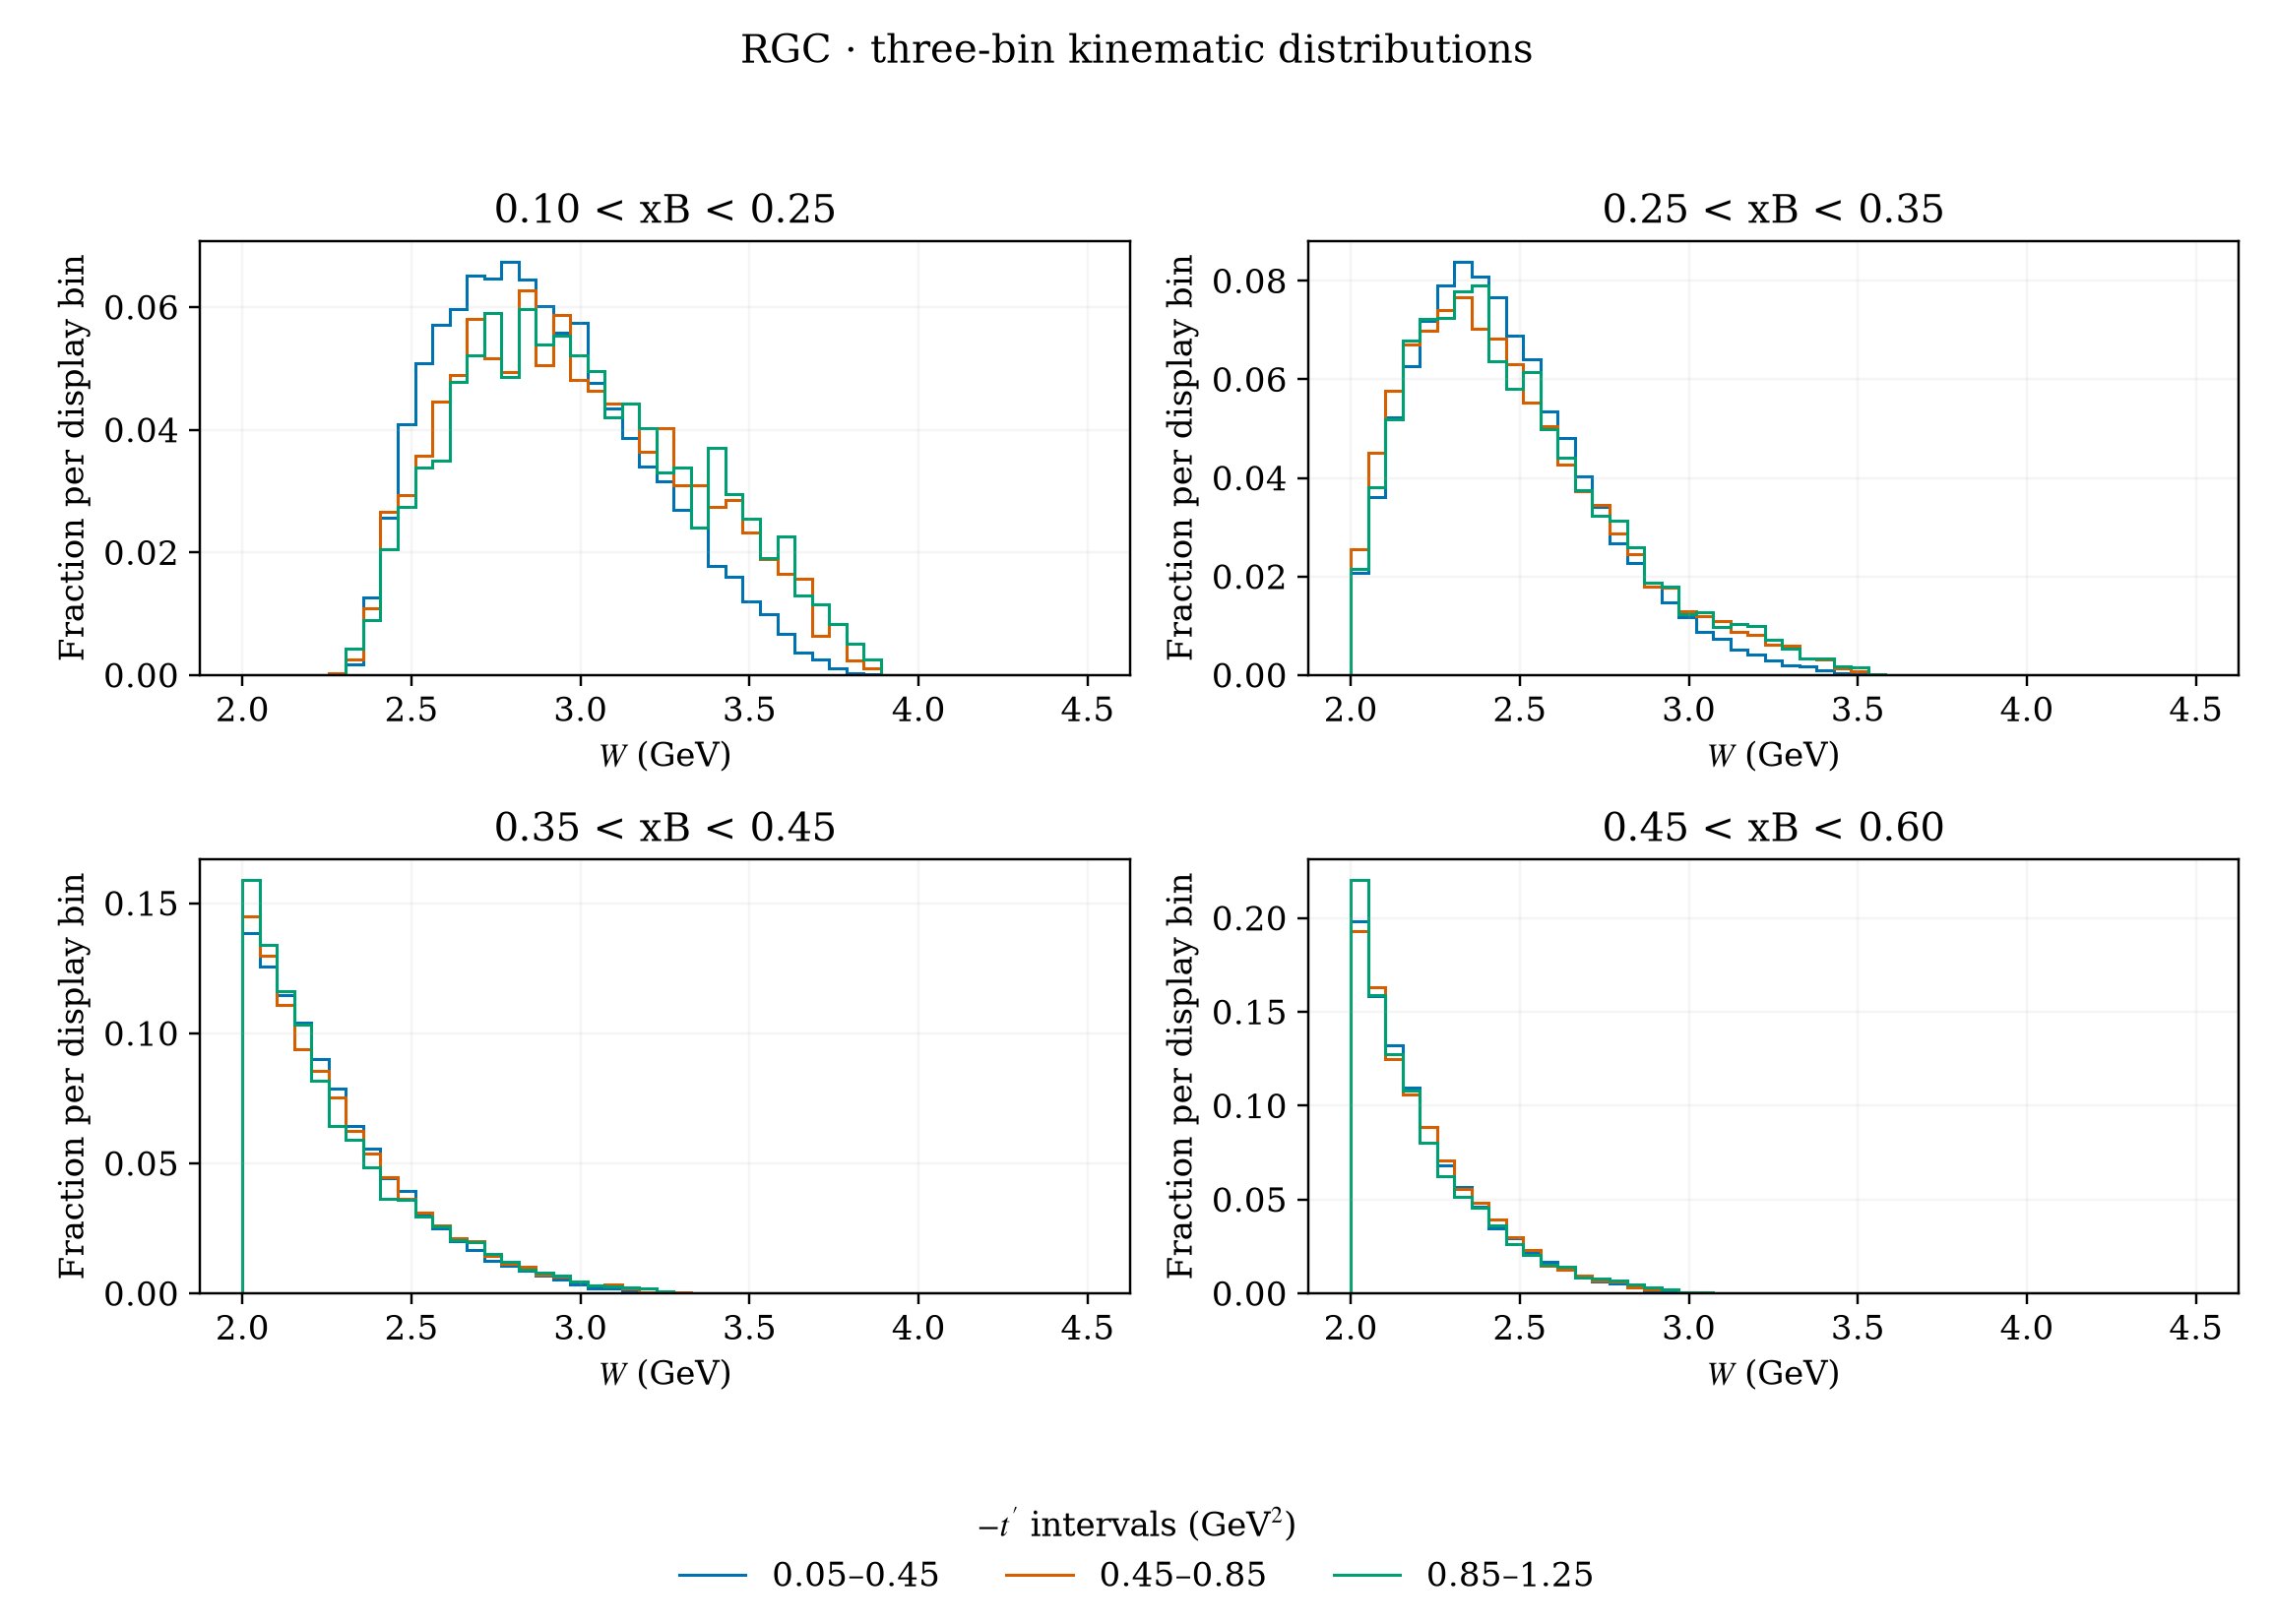
\includegraphics[width=\linewidth]{figures/results/RGC_W_three_bin_2x2.png}
\caption{RGC distributions in the three merged target-sector bins. Each curve is normalized over its displayed range. The legends give the $-t^\prime$ intervals in GeV$^2$.}\label{fig:release_kin_RGCW}
\end{figure}
\clearpage
\begin{figure}[p]\centering
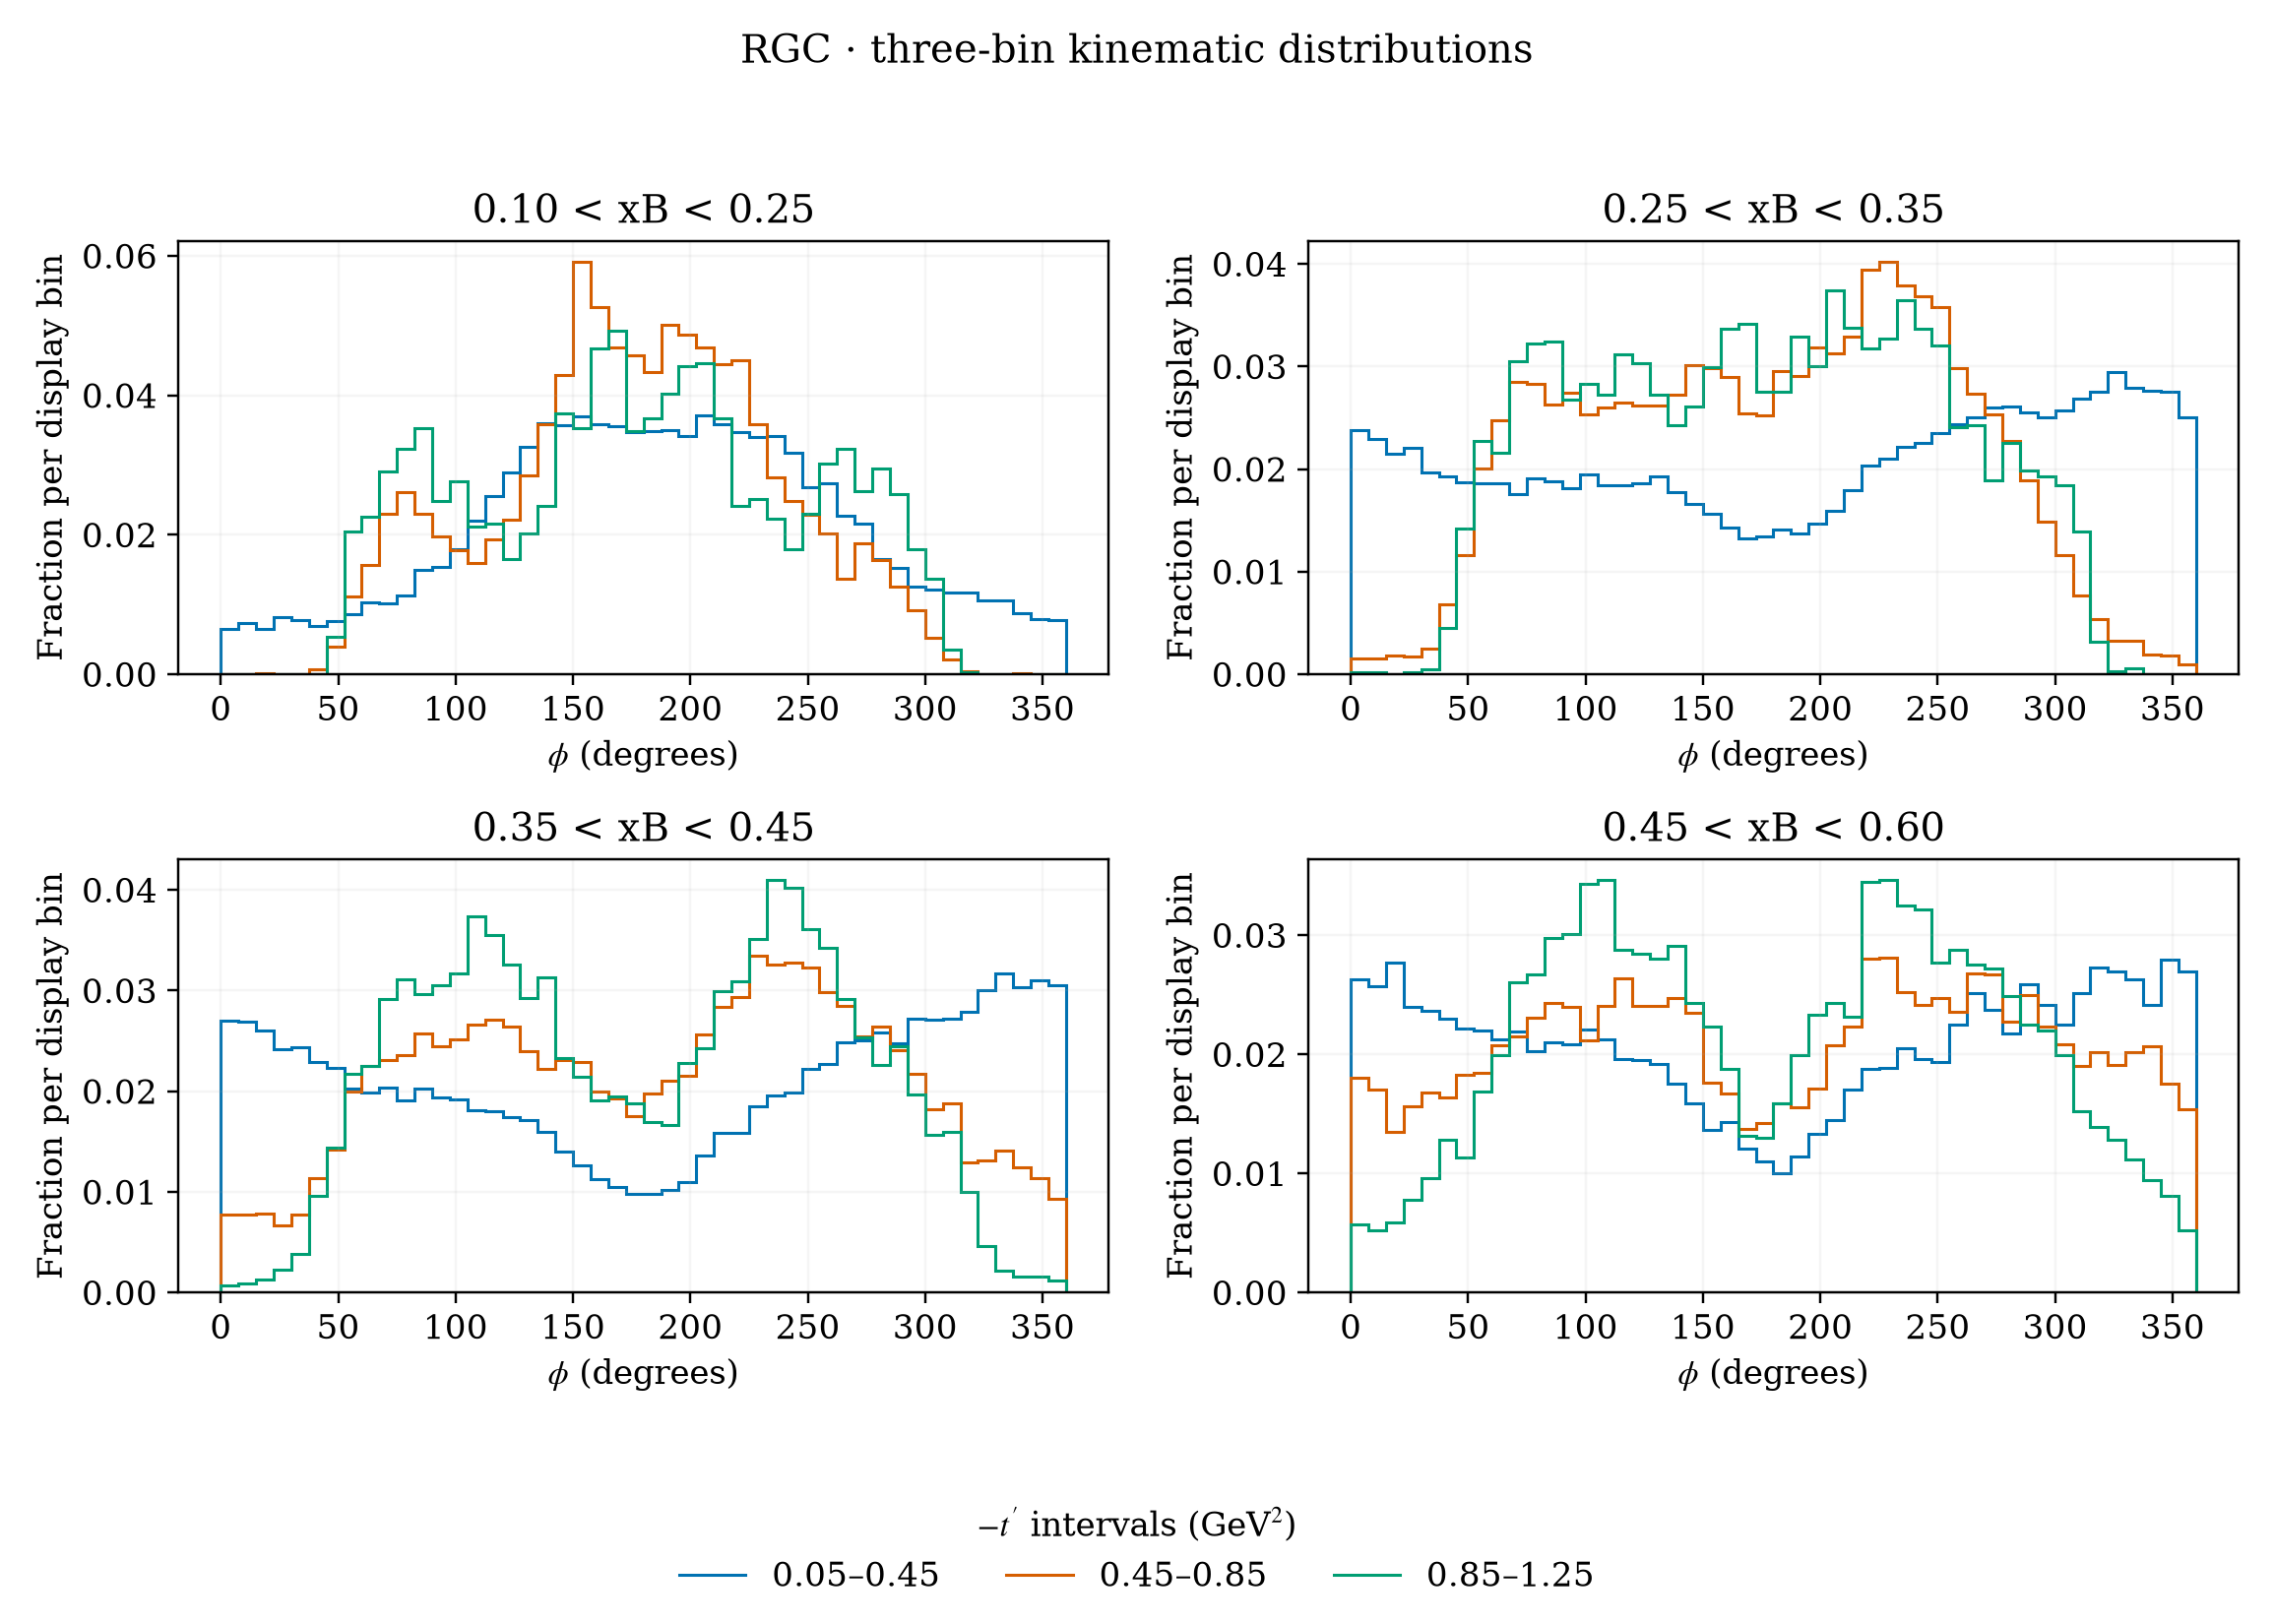
\includegraphics[width=\linewidth]{figures/results/RGC_phi_three_bin_2x2.png}
\caption{RGC distributions in the three merged target-sector bins. Each curve is normalized over its displayed range. The legends give the $-t^\prime$ intervals in GeV$^2$.}\label{fig:release_kin_RGCphi}
\end{figure}
\clearpage
